\documentclass{article}

% neurips_2026.sty, used unmodified, submission (anonymous) mode.
% Provenance: the official download URLs on neurips.cc/media.neurips.cc were
% unreachable (404) on 2026-08-31; this copy was obtained from a public
% mirror of the official style (ProvidesPackage 2026-01-29 NeurIPS 2026
% submission/camera-ready style file). Before camera-ready, re-verify this
% file byte-for-byte against the official NeurIPS 2026 release.
\usepackage[dblblindworkshop,final]{neurips_2026}
\workshoptitle{SLMs for Agentic Systems, Paris, France, 2026}

\usepackage[utf8]{inputenc}
\usepackage[T1]{fontenc}
\renewcommand{\ttdefault}{lmtt}  % Latin Modern typewriter (Type 1) instead of bitmap EC typewriter
\usepackage{hyperref}
\hypersetup{hidelinks}
\usepackage{url}
\usepackage{booktabs}
\usepackage{amsfonts,amsmath}
\usepackage{nicefrac}
\usepackage{microtype}
\usepackage{graphicx}
\usepackage{xcolor}
\usepackage{etoolbox}
\raggedbottom
\renewcommand{\topfraction}{0.95}\renewcommand{\textfraction}{0.05}\renewcommand{\floatpagefraction}{0.9}
% tighten float/text separation (page budget)
\setlength{\textfloatsep}{9pt plus 2pt minus 3pt}
\setlength{\floatsep}{7pt plus 2pt minus 2pt}
\setlength{\intextsep}{8pt plus 2pt minus 2pt}

\usepackage{amsthm}
\newtheorem{definition}{Definition}
\newtheorem{proposition}{Proposition}
\newtheorem{remark}{Remark}
\newcommand{\stmp}{S_{\text{temporal}}}
\newcommand{\Gagg}{\bar G}
\newcommand{\iet}{\tau}
\newcommand{\qrr}{q_{RR}}

% Title alternatives considered for SLM-Agents fit (author decision):
%  (a) Scaffold Does Not Buy Temporal Fidelity: State Fidelity Is Not Process Fidelity in Efficient LM-Agent Simulators
%  (b) Does Smaller Buy Realism? State Fidelity Is Not Process Fidelity in Efficient LM-Agent Simulators
\title{From Structural to Temporal Fidelity in Dynamic Graph Generation}

\author{%
  Parham Hamouni\\
  Toronto Metropolitan University\\
  \texttt{parham.hamouni@torontomu.ca}
  \And
  Ebrahim Bagheri\\
  University of Toronto\\
  \texttt{ebrahim.bagheri@utoronto.ca}
}


\begin{document}
\maketitle
\begin{abstract}
Language model agents are increasingly used to simulate dynamic text attributed
graphs, but it is unclear whether more efficient systems preserve the temporal
dynamics of real interaction streams. Existing evaluations mainly measure
\emph{state fidelity} through structural, textual, and marginal timing
statistics, while applications such as forecasting and intervention analysis
also require \emph{process fidelity}. We show that statistics based only on
marginal behavior cannot distinguish a process that preserves event ordering
from one that destroys temporal dependence. We therefore introduce R2O, a
likelihood-free framework that evaluates temporal fidelity along three
dimensions. \emph{Rate} measures the pace of activity, \emph{Rhythm} measures
the distribution of inter-event times, and \emph{Order} measures dependence
between consecutive intervals. Each discrepancy is calibrated against
variation between matched windows of real data. Across three scaffold configurations, three backbones, and four datasets,
R2O reveals a consistent separation between structural and temporal fidelity.
Configurations that improve structural realism do not consistently move closer
to the real temporal process, and no preregistered configuration reproduces
the temporal dependence observed in the real streams. Changing the language model backbone changes
which temporal properties are better matched, but does not yield consistent
agreement across Rate, Rhythm, and Order. These results show that structural
fidelity alone is insufficient for evaluating efficient dynamic graph
generation.
\end{abstract}

\section{Introduction}
\label{sec:intro}

Language model agents are increasingly used to simulate evolving social and
interaction systems represented as dynamic text attributed graphs
\citep{zhang2024dtgb,ji2025gag,peng2025gdgb,ji2026graphia}. Such systems combine
language model decisions with interaction history, memory, and tool use to
generate both graph structure and text over time. Simulation over large
populations and long horizons makes inference cost a central design constraint,
which motivates the use of smaller language model backbones
\citep{belcak2025slm,yang2025qwen3}. In practice, reduced backbone capacity can
also be paired with richer agent scaffolding. This creates an important
question for small model agent systems. Whether a cheaper backbone, additional
scaffolding, or their combination preserves the process that the agents are
intended to simulate cannot be determined from efficiency or output realism
alone.

This issue is different from asking whether a small model can reproduce the
same individual decisions or final graph statistics as a larger model. In an
agent simulation, backbone and scaffold choices are repeatedly applied as the
system evolves, so apparently local differences can alter when interactions
occur and how subsequent activity depends on prior events. A configuration can
therefore produce plausible agents and realistic graph structure while
generating a different temporal process. For efficient agent systems, the
relevant tradeoff is consequently not only quality against computational cost,
but fidelity of the generated process against computational cost. Evaluating
that tradeoff requires measurements that remain meaningful when backbone and
scaffold choices change the dynamics without substantially changing the
resulting states.

Existing graph generation evaluation does not directly provide such a test.
Static graph generators are primarily compared through structural statistics
such as degree, clustering, and motifs
\citep{you2018graphrnn,liao2019gran,obray2022evaluation}. DyTAG systems extend
this evaluation to generated text, activity trajectories, and marginal
timestamp statistics \citep{ji2025gag,peng2025gdgb,ji2026graphia}. Related
language model social simulations have begun to model temporal behavior more
explicitly. These approaches
demonstrate the importance of temporal behavior, but the literature summarized
in Appendix~\ref{app:landscape} does not provide an evaluation framework for
LM agent DyTAG streams that jointly tests order sensitive event dependence and
interprets the resulting discrepancy relative to variation between comparable
real streams.

We refer to agreement on generated structure, text, and marginal activity
statistics as \emph{state fidelity}. For many uses of simulation, matching the
state is not sufficient. Forecasting, intervention analysis, and synthetic
event generation depend on how future events vary with preceding history. We
call agreement in this conditional evolution \emph{process fidelity}. For a
graph sequence $G_{1:T}$, the distinction is between properties of the
marginal distribution $P(G_t)$ and properties of the conditional distribution
$P(G_t\mid G_{<t})$. This distinction is particularly relevant when comparing
small model backbones and agent scaffolds because two configurations can agree
on the states they produce while differing in how those states evolve.

Marginal agreement does not identify temporal dependence. Permuting an actor's
inter-event times preserves its event count, inter-event time distribution,
and statistics computed from the time aggregated graph while changing the
order in which activity unfolds. We formalize this observation and show that
statistics depending only on the aggregated graph or unordered inter-event
times are invariant to this transformation. Process fidelity therefore
requires at least one statistic that responds to event order.

We introduce R2O, a likelihood-free framework that evaluates temporal process
fidelity along three separate axes. \emph{Rate} measures activity pace,
\emph{Rhythm} measures the inter-event time distribution, and \emph{Order}
measures dependence between consecutive intervals. Each discrepancy is
interpreted relative to variation between matched windows of the real stream.
We establish order sensitivity, separation among the three axes, and finite
sample calibration, and validate these properties with shuffled and memoryless
controls. Proofs and synthetic validation are provided in
Appendix~\ref{app:proofs}.

Our contributions are (1) a formal distinction between state and process
fidelity for LM agent DyTAG simulation, together with an invariance result
showing why structural and marginal timing statistics cannot detect loss of
event order, (2) R2O, which separately evaluates activity rate, inter-event
time distributions, and temporal dependence relative to variation within the
real data, and (3) an evaluation across scaffold configurations, backbones,
and datasets that tests whether structural improvements obtained through
backbone and scaffold choices also preserve temporal dynamics. Empirically,
structural improvements do not reliably reduce temporal discrepancies,
marginal timing agreement need not imply agreement in event dependence, and
changing the language model backbone does not consistently resolve the gap
across Rate, Rhythm, and Order. These results show why process fidelity is a
necessary consideration when evaluating efficient agent simulation.

\section{Requirements for measuring process fidelity}
\label{sec:requirements}

Temporal process fidelity requires more than agreement in aggregate properties.
Human interaction streams are bursty and temporally correlated
\citep{barabasi2005origin,goh2008burstiness,karsai2018bursty}, and streams with
identical marginal statistics can differ in that dependence
\citep{malmgren2008poissonian,holme2012temporal}. An evaluation must therefore
respond to event order, distinguish sources of temporal error, and provide a
scale on which discrepancies can be interpreted.

\subsection{Event streams and classes of statistics}

An event stream is
$E=((u_i,v_i,x_i,t_i))_{i\le n}$, where $u_i$ and $v_i$ denote the
interacting actors, $x_i$ is the associated text, and $t_i$ is a
non decreasing timestamp. For actor $u$, let
$\iet^u_j=t^u_{j+1}-t^u_j$ denote its $j$th inter-event time (IET),
$T^u$ the multiset of its IETs, $T=\biguplus_u T^u$ the pooled IET
multiset, and $\Gagg(E)$ the time aggregated graph.

\begin{definition}[State, marginal timing, and dependence statistics]
\label{def:state}
A statistic is a \emph{state statistic} if it is computed from generated
states without using the order of an actor's IETs. It is a \emph{marginal
timing statistic} if it depends on timing only through the multisets
$\{T^u\}_u$, and a \emph{dependence statistic} if changing the order of IETs
within an actor can change its value.
\end{definition}

Structural statistics such as degree MMD, clustering, and motifs are widely
used to compare generated and real graphs
\citep{you2018graphrnn,liao2019gran,obray2022evaluation}. DyTAG generators also
compare text similarity, activity trajectories, and count based temporal
summaries \citep{ji2025gag,peng2025gdgb,ji2026graphia}. These are state
statistics because they do not use IET order. Pooled IET KS, $W_1$ on log
IETs, the burstiness gap $|\Delta B|$, and node rhythm divergence are marginal
timing statistics \citep{goh2008burstiness,karsai2012universal}. Memory $M$
and global lag 1 IET autocorrelation are dependence statistics because they
use consecutive intervals. We use \emph{state fidelity} for agreement on state
and marginal timing properties and \emph{process fidelity} for agreement in
temporal dependence. A broader comparison is in Appendix~\ref{app:landscape}.

\subsection{Requirement 1: sensitivity to event order}

Agreement in marginal timing does not determine temporal dependence. Two
processes can have the same IET distributions and time aggregated graph
statistics while differing in how successive events depend on their history.

\begin{proposition}[Non identification of temporal dependence]
\label{prop:nonident}
Let $F$ be any IET distribution with finite variance. Let $P_0$ generate each
actor's IETs independently from $F$, and let $P_\rho$ generate them from a
stationary Gaussian copula AR(1) process with the same marginal $F$ and
parameter $\rho\in(0,1)$. If partner and text choices are identical and
independent of event timing, then $P_0$ and $P_\rho$ have identical actor level
IET marginals, identical burstiness, and identical distributions for every
state statistic, while $M(P_\rho)>0=M(P_0)$.
\end{proposition}

The same limitation can be exposed directly on an observed stream. Let
$\varsigma(E)$ independently permute the IET sequence of each actor.

\begin{proposition}[Shuffle invariance]
\label{prop:shuffle}
Statistics that depend only on $\Gagg(E)$ or on the unordered IET multisets
$\{T^u\}_u$ are unchanged by $\varsigma$. For an actor with $k_u\ge3$ IETs,
\[
\mathbb{E}[M^u(\varsigma(E))\mid E]=O(1/k_u).
\]
Thus, a generator can reproduce each actor's IET marginal while carrying no
temporal memory and remain indistinguishable under order invariant statistics.
\end{proposition}

Process evaluation must therefore include at least one statistic that changes
when event order changes. The construction and proofs of both propositions are
provided in Appendix~\ref{app:proofs}.

\subsection{Requirement 2: separation of failure modes}

Temporal error can arise in different ways. A simulator may generate events at
the wrong overall rate, reproduce the wrong distribution of inter-event times,
or fail to reproduce dependence between consecutive intervals. These errors
cannot be diagnosed reliably after they are collapsed into a scalar.

\begin{proposition}[Separation under rate changes]
\label{prop:separation}
Under a global rescaling $\iet\mapsto a\iet$, burstiness $B$, memory $M$, and
lag 1 autocorrelation are invariant. Pooled IET KS and node rhythm KS are not
invariant, and
\[
\left|W_1(\log a\iet,\log\iet')-W_1(\log\iet,\log\iet')\right|
\le |\log a|.
\]
Equality holds when the two unscaled log IET distributions coincide (the case
checked in Table~\ref{tab:synthetic-validation}, where $W_1 = 2.996 = \log 20$);
it need not hold for distributions of the same shape at different locations. Hence
$\log(T_g/T_r)$ isolates rate, $B$ and $W_1(\log\iet)$ characterize
marginal timing up to the stated rate term, and $M$ and lag 1 autocorrelation
characterize dependence.
\end{proposition}

Rate, marginal timing, and temporal dependence should therefore be reported
separately. These three failure modes define the \emph{Rate}, \emph{Rhythm},
and \emph{Order} axes of R2O. The proof is given in
Appendix~\ref{app:proofs}.

\subsection{Requirement 3: calibration against real data variability}

Raw discrepancy values do not have a common interpretation across datasets or
evaluation windows. The same KS distance, Wasserstein distance, or change in
memory may reflect ordinary variation in one dataset but a mismatch
in another. Standard point process diagnostics can obtain a reference
distribution from a specified conditional intensity
\citep{ogata1988statistical,brown2002timerescaling}, but the LM agent DyTAG
generators considered here do not expose a tractable conditional event
likelihood \citep{ji2025gag,peng2025gdgb,ji2026graphia}. We therefore
interpret each simulator to real discrepancy relative to the same discrepancy
measured between matched windows of the real stream.

For a simulator to real discrepancy $D^{SR}$, let $D^{RR}_{1:N}$ denote the
same discrepancy computed between $N$ matched pairs of real windows and define
\[
q_{\mathrm{RR}}=
\frac{1+\#\{i:D^{RR}_i\ge D^{SR}\}}{N+1}.
\]

\begin{proposition}[Finite sample calibration]
\label{prop:calibration}
If $D^{SR}$ is exchangeable with $D^{RR}_{1:N}$, then
$\Pr(q_{\mathrm{RR}}\le\alpha)\le\alpha$ for every $\alpha\in[0,1]$.
Moreover, $q_{\mathrm{RR}}=1/(N+1)$ exactly when $D^{SR}$ exceeds every real
to real discrepancy.
\end{proposition}

The calibration places each simulator discrepancy on the scale of variability
already present in the observed process. R2O applies it separately to each
axis rather than combining heterogeneous discrepancies into a single score.
The proof and matching details are given in Appendices~\ref{app:proofs}
and~\ref{app:instrument}.

These requirements define how R2O should distinguish different forms
of temporal mismatch. Structural improvements need not reduce temporal
discrepancies, agreement on Rhythm need not imply agreement on Order, and the
three axes may favor different configurations. A discrepancy should also remain
outside the matched real reference after accounting for plausible measurement
artifacts. Section~\ref{sec:results} evaluates these patterns empirically.

\section{The R2O framework}
\label{sec:r2o}

Given a generated stream $E_g$ and a corresponding real stream $E_r$ (complete
streams, or matched continuations of a common observed history), R2O computes
discrepancies along Rate, Rhythm, and Order and calibrates each against
matched real data segments.\label{sec:r2o_protocol} It does not prescribe how
$E_g$ is produced, so it scores conditioned and closed loop generation alike,
keeping generation and evaluation separate.

\subsection{Rate, Rhythm, and Order}
\label{sec:r2o_axes}

\noindent \textbf{Rate}
Rate measures agreement in the pace of activity. For generated and
real durations $T_g$ and $T_r$,
\[
D_{\mathrm{Rate}}=\left|\log\frac{T_g}{T_r}\right|.
\]
The discrepancy is zero when the two time scales agree and changes under
uniform rescaling while the Order statistics remain invariant.

\noindent \textbf{Rhythm}
Rhythm measures agreement in the marginal distribution of IETs without using
their sequential order. At the population level, R2O uses pooled IET KS,
Wasserstein distance on log IETs, and the burstiness difference $|\Delta B|$
\citep{goh2008burstiness,karsai2012universal}. At the actor level, node rhythm
divergence is
\[
D_{\mathrm{node}}=
\operatorname*{median}_{u}\mathrm{KS}\!\left(T_g^u,T_r^u\right).
\]
The pooled statistics characterize population timing, while node rhythm
preserves actor identity and can expose discrepancies hidden by pooling.

\noindent \textbf{Order}
Order measures agreement in dependence between consecutive intervals. R2O
uses $D_M=|M_g-M_r|$ and
$D_{\rho}=|\rho_{1,g}-\rho_{1,r}|$. Unlike Rhythm, these statistics change
when the same intervals are reordered. They distinguish streams that
share an IET distribution but differ in temporal dependence, which is the
failure mode established by Propositions~\ref{prop:nonident}
and~\ref{prop:shuffle}. R2O does not combine Rate, Rhythm, and Order into a scalar because
agreement on one axis need not imply agreement on others.

\subsection{Calibration with real data}
\label{sec:r2o_calibration}

Each discrepancy is interpreted relative to matched real segments. The same R2O
statistic is computed across observed window pairs to form a real reference
distribution, and the simulator is located within its upper tail using
$q_{\mathrm{RR}}$. A small value indicates a discrepancy larger than typical
variation in the real process. Matching and controls for timestamp ties,
scheduler quantization, actor activity, and window selection are described in
Appendix~\ref{app:instrument}.

\noindent \textbf{Construction of the real reference}
R2O builds the reference from pairs of 10,000 edge real windows matched on
duration, actor count, edges per actor, and median positive IET, using up to 60
pairs per dataset with reuse of any window capped at three. We report
$q_{\mathrm{RR}}$ together with a standardized discrepancy $Z_D$ in units of
real variation. The calibration compares each simulator against
comparable real activity regimes rather than arbitrary windows. Full details
are in Appendix~\ref{app:instrument}.

\begin{figure}[!t]
\centering
\begin{minipage}[t]{0.48\textwidth}
\centering
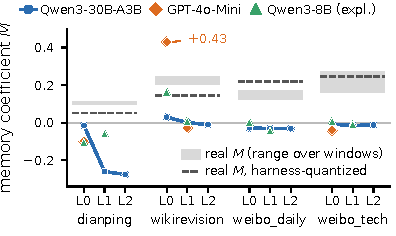
\includegraphics[width=\linewidth]{fig1_memory.pdf}
\caption{\textbf{Order: memory coefficient $M$ by dataset and scaffold level.}
Grey bands give the range of real $M$ over matched windows; dashed lines give
real $M$ after harness quantization (Appendix~\ref{app:instrument}). Markers
are generated $M$ for the Qwen3-30B-A3B ladder (L0/L1/L2), GPT-4o-Mini, and
the exploratory Qwen3-8B cells. No Qwen3-30B-A3B cell reaches the real band;
GPT-4o-Mini on wikirevision L0 overshoots it ($M = +0.43$), and the closest
point, the exploratory Qwen3-8B wikirevision L0 cell ($Z_{|\Delta M|} = +1.2$),
does not survive matched horizon rescoring (Table~\ref{tab:matched-horizon};
\S\ref{sec:backbone}). Values: Appendix~\ref{app:tables}.}
\label{fig:memory}
\end{minipage}
\hfill
\begin{minipage}[t]{0.48\textwidth}
\centering
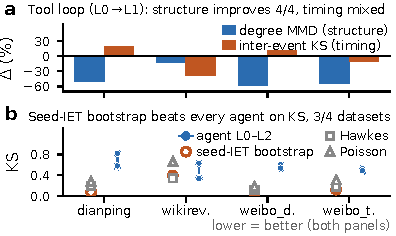
\includegraphics[width=\linewidth]{fig2_decoupling.pdf}
\caption{\textbf{Structure versus timing.} (a) Percent change from L0 to L1 in
degree MMD (structure) and inter-event KS (Rhythm); negative is better. Structure
improves on all four datasets while Rhythm moves in both directions. (b)
Inter-event KS of the agent cells against the Poisson, seed-IET bootstrap, and
Hawkes timing baselines; the bootstrap, which has no temporal dependence by
construction, is lowest on three of four datasets. Values:
Appendix~\ref{app:tables}.}
\label{fig:decoupling}
\end{minipage}
\end{figure}

\noindent \textbf{Synthetic validation of axis separation}
Synthetic controls verify the intended separation before model evaluation.
Shuffling a dependent stream preserves its IET distribution and burstiness
while reducing memory from $0.164$ to $-0.007$; an independent renewal process
with the same marginal behaves similarly. Rescaling time by a factor of 20
leaves memory at $0.164$ while moving IET KS to $0.686$ and log Wasserstein
distance to $2.996$. The complete validation is in Appendix~\ref{app:proofs}.

\section{Experiments and findings}
\label{sec:results}


We evaluate R2O on \texttt{dianping}, \texttt{wikirevision},
\texttt{weibo\_daily}, and \texttt{weibo\_tech}, the four GDGB datasets with
suitable temporal information \citep{peng2025gdgb}; GRAPHIA lacks continuous
timestamps (Appendix~\ref{app:graphia}). The primary experiments compare L0, which reproduces GAG General \citep{ji2025gag}, L1,
which adds tool use, and L2, which additionally includes a memory module
(distinct from the memory coefficient $M$ of \S\ref{sec:r2o_axes}). Qwen3-30B-A3B
is the primary backbone, GPT-4o-Mini provides matched backbone comparisons, and
Qwen3-8B is exploratory; the primary analysis contains 16 preregistered
configurations. Each run starts from a real prefix and is scored against the
corresponding real continuation, alongside Poisson, empirical IET bootstrap,
and Hawkes timing baselines. For Qwen3-8B, L0 uses 1.9 to 2.8 language model
calls per event and L1 uses 2.5 to 4.7, with 1.6 to 2.4 times more prompt
tokens (details: Appendix~\ref{app:setup}).

\noindent \textbf{R2O separates structural improvement from process fidelity}
From L0 to L1, degree MMD improves on all four datasets by $43.8\%$ on
average, while inter-event KS changes in mixed directions, from $-38.0\%$ to
$+18.5\%$ across datasets ($-4.8\%$ on average; Figure~\ref{fig:decoupling}). Even the best structural configuration on each
dataset remains outside the corresponding real reference on temporal measures.
On the representative wikirevision window (GPT-4o-Mini;
Appendix~\ref{app:instrument}), the log duration ratio also worsens from
$3.83$ to $4.44$, or approximately $46$ to $85$ times the real duration:
structural improvement does not imply temporal process fidelity.

\noindent \textbf{The Order axis detects discrepancies that Rhythm cannot identify}
Real memory coefficients range from $0.10$ to $0.27$, but none of the 16 preregistered
 configurations reproduces this dependence. Across the 12 Qwen3-30B-A3B
 configurations, memory ranges from $-0.28$ to $0.03$, and every
configuration lies outside the real reference range on the memory discrepancy
(Figure~\ref{fig:memory}). Rhythm fails less uniformly: actor level rhythm divergence lies inside the
real reference ($|Z| \le 2$) on 7 of the 16 configurations, so a simulator can approach
actors' IET distributions without reproducing dependence between successive
intervals. This is the distinction for which Order is
needed.

\noindent \textbf{The R2O axes reveal different effects of the language model backbone}\label{sec:backbone}
Matched Qwen3-30B-A3B and GPT-4o-Mini comparisons improve some temporal
measures while worsening others, and exploratory Qwen3-8B runs show the same
pattern. The only 8B configuration approaching real memory also has the
largest marginal timing discrepancy in that set, and matched horizon controls
place memory near the shuffled value in all eight exploratory arms. Backbone
changes therefore alter which temporal properties are matched without
consistent improvement on Rate, Rhythm, and Order.

\noindent \textbf{The timing baselines show why Rhythm alone is insufficient}
The empirical IET bootstrap samples intervals independently from the observed
seed distribution, retaining marginal timing but not temporal dependence. It
outperforms every agent configuration on inter-event KS on three of four
datasets (Figure~\ref{fig:decoupling}; $0.065$ to $0.122$ versus $0.468$ to
$0.559$ for the best agent). Generating neither structure nor text, it is
diagnostic: it instantiates Proposition~\ref{prop:nonident}, with global lag 1
autocorrelation $-0.002$ to $+0.002$ (20 seeds) against real $0.22$ to $0.36$,
so strong Rhythm coexists with complete failure on Order. The Hawkes baseline,
in contrast, partially recovers the temporal dependence observed in the real
data, with lag 1 autocorrelation of $0.14$ to $0.31$ against $0.22$ to $0.36$
in the real sequences, so the seed prefix contains recoverable temporal
dependence that a seed-conditioned generator can partially reproduce; the
Qwen3-30B-A3B agent streams fall below the real value in 10 of 12 cells and
overshoot it in the other two (Appendix~\ref{app:tables}).




\begin{figure}[t]
\centering
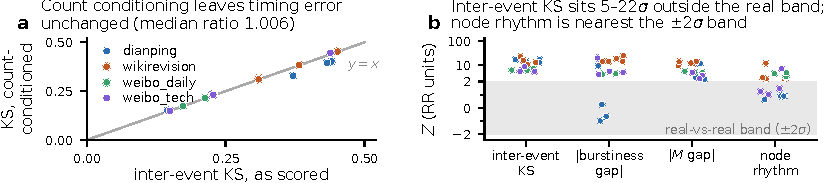
\includegraphics[width=\linewidth]{figA_controls.pdf}
\caption{\textbf{R2O under measurement controls.} Count matching leaves
marginal timing largely unchanged, while standardized temporal discrepancies
remain outside the matched real reference.}
\label{fig:controls}
\end{figure}

\noindent \textbf{R2O findings remain stable under measurement controls}
Matching actor level event counts has little effect on marginal timing, and the
standardized R2O scores remain outside variation across matched real windows
(Figure~\ref{fig:controls}). The Order discrepancy also persists after controls
for timestamp ties, scheduler quantization, and evaluation window selection;
in particular, imposing the generation scheduler on the real stream changes
real memory by between a $49\%$ reduction and a $39\%$ increase yet leaves it
above every Qwen3-30B-A3B generated value on all four datasets, so neither
the harness nor the scoring procedure explains the gap (controls:
Appendix~\ref{app:instrument}; proofs: Appendix~\ref{app:proofs}).

\noindent \textbf{Limitations}\label{sec:limitations}
The evaluation covers one DyTAG system lineage and shared generation pipeline,
with teacher forced generation and four datasets. Teacher forcing is expected to
understate Order error, since dependence errors cannot compound when real
history is re-injected; Rate and Rhythm could move in either direction under
closed loop rollout, which is what the preregistered roll forward test
measures. The scheduler control rules out timestamp quantization alone as the
source of the Order gap, but whether the language model or the scheduler
decides event timing remains open; the preregistered timing locus test
(Appendix~\ref{app:followups}) addresses this. Order uses lag 1 statistics ($M$, $\rho_1$) and can miss longer
range or nonlinear dependence. Configurations are single archived runs rather
than replicated seeds, some terminate before the nominal horizon, and API
served backbones carry provider side serving opacity. Real to real calibration
measures variation across observed windows but does not estimate generation
seed uncertainty; $q_{\mathrm{RR}}$ is an empirical tail position, not a
hypothesis test value, with floor $1/14$ on \texttt{weibo\_tech} (13 pairs),
where the conclusion rests on $Z$. Downstream consequences for forecasting or
intervention analysis are not measured here. Additional limitations and
serving details are in Appendix~\ref{app:limitations}.

\section{Conclusion}
State fidelity is not process fidelity. Statistics computed from marginal
behavior are invariant to the within actor reordering that erases temporal
dependence, so a simulator can match structure, text, counts, and inter-event
time distributions while generating a process unlike the real one. R2O makes
the missing axis measurable: it separates Rate, Rhythm, and Order and reports
each against the variability between matched real windows. Applied to an
efficient LM agent lineage, it shows that scaffolding improves structural
fidelity without repairing temporal dependence, that backbone choice moves the
deficit rather than removing it, and that a parameter free bootstrap of seed
inter-event times matches the real Rhythm better than every agent
configuration on three of four datasets. Evaluations of agent based simulators
intended for forecasting or intervention analysis should therefore include an
order sensitive, real reference calibrated test alongside state metrics.

\begin{ack}
This research was supported by the Natural Sciences and Engineering Research
Council of Canada (NSERC), grant number RGPIN-2024-04733.
\end{ack}

\clearpage
\bibliographystyle{plainnat}
\bibliography{refs}

\clearpage
\appendix

\section{Experimental details and reproducibility}
\label{app:setup}
\label{app:experimental}

\subsection{Datasets and configurations}

The experiments use \texttt{dianping}, \texttt{wikirevision},
\texttt{weibo\_daily}, and \texttt{weibo\_tech} from GDGB. These are the four
datasets used for the temporal analysis in the main paper. All R2O statistics
are computed from event timestamps after the same preprocessing used by the
generation pipeline. Dataset access and preprocessing follow the GDGB release.

The primary analysis contains 16 preregistered configurations. Twelve use
Qwen3-30B-A3B and cover the four datasets under L0, L1, and L2. L0 reproduces
GAG General, L1 adds tool use, and L2 additionally includes memory. Four
archived GPT-4o-Mini configurations provide matched backbone comparisons on
\texttt{dianping} L0, \texttt{wikirevision} L0 and L1, and
\texttt{weibo\_tech} L0. A separate exploratory analysis contains eight
Qwen3-8B configurations covering L0 and L1 on all four datasets. Exploratory
results are excluded from statements that refer to the 16 preregistered
configurations.

\subsection{Generation protocol}

Each run conditions on a real prefix containing 1,000 edges and generates a
continuation of approximately 9,000 events in rounds of 50 events. The main
evaluation uses the corresponding real continuation from the inherited
10,000-edge evaluation window. Reference statistics are computed from the
matched real slots of the same window.

Several archived runs terminate before the nominal horizon. The archived
Qwen3-30B-A3B runs for \texttt{weibo\_tech} L1,
\texttt{weibo\_tech} L2, and \texttt{weibo\_daily} L2 are shorter than the
nominal run. The \texttt{weibo\_daily} L2 structural evaluation is excluded
because the archived structural output is contaminated, while its timing
statistics use the archived run produced before contamination. The
GPT-4o-Mini run for \texttt{wikirevision} L1 contains 7,232 events and the
GPT-4o-Mini run for \texttt{weibo\_tech} L0 contains 200 generated events.
Its timing statistics use the same matched-slot procedure at the available
horizon, while structural statistics are unavailable because the structural
evaluation lane was not run for such a short stream. Configuration-level
numbers of scored events are reported in Table~\ref{tab:artifact-controls}.

The exploratory Qwen3-8B L1 runs were stopped at round boundaries because of
generation time. Their lengths range from 4,900 to 5,696 events. For
comparisons between exploratory L0 and L1, we therefore also report a
matched horizon analysis in which the corresponding L0 stream is truncated to
the L1 event count and rescored using the same procedure.

\subsection{Backbones, serving, and efficiency}

Qwen3-30B-A3B (checkpoint \texttt{Qwen3-30B-A3B-Instruct-2507-FP8}) is served
locally with vLLM 0.20.0 (FP8 weights, tensor parallel size 1, that is, one
GPU per server instance, 32,768-token context limit) on a server with eight
NVIDIA RTX 6000 Ada (48\,GB) GPUs, 64 CPU cores, and 710\,GB RAM, which also
ran the agent harness. GPT-4o-Mini (\texttt{gpt-4o-mini-2024-07-18}, version pinned) is
accessed through a commercial API gateway; its harness ran on a 128-core,
541\,GB server whose two NVIDIA RTX A6000 (48\,GB) GPUs serve only the
retrieval embedding model. The provider does not expose its serving stack or
a determinism guarantee, so API runs are not used to estimate variance for the
local model. The exploratory Qwen3-8B runs use the same API gateway with
provider reasoning disabled. All three backbones use the same decoding
configuration in the generation harness (recorded in the harness model
configuration of every cell): temperature 0.3 and at most 1,024 generated
tokens per call. Wall-clock generation times were not retained in
the run archive; per-call token and call counts are retained for the
exploratory grid (below). All scoring and analysis is CPU only.

For the exploratory Qwen3-8B grid, API accounting gives 1.9 to 2.8 LM calls per
event for L0 and 2.5 to 4.7 calls per event for L1. L1 uses 1.6 to 2.4$\times$
more prompt tokens per event than L0. The resulting cost is
\$4.48 to \$7.77 per cell and \$46.78 for the complete exploratory grid.
Code, score tables, and the verification gate are available at
\url{https://github.com/parhamouni/r2o-process-fidelity}. Per-call token usage and call counts are retained in the supplementary
material.

\subsection{Timing baselines}

Three timing baselines use only the 1,000-edge seed prefix. The Poisson
baseline estimates a constant event rate from the seed. The empirical IET
bootstrap samples seed inter-event times independently with replacement. The
Hawkes baseline fits an exponential Hawkes process to the seed by maximum
likelihood. These baselines generate event times only and do not generate graph
structure or text. Reported baseline means and standard deviations use 20
simulation seeds.

\subsection{Registration and reproducibility}
\label{app:repro}

The primary configuration set and the main R2O analyses were preregistered.
The Qwen3-8B arm was added after registration and is labeled exploratory
throughout the paper.

All analysis code, per configuration scores, matched real-window construction,
the scheduler and count-conditioning controls, figure and table generation
scripts, and a verification gate that recomputes every statistic reported in
the paper from the committed score files are provided in the
supplementary material and in the public repository. The repository data are read only under the analysis
scripts, and every figure and table is regenerable from the committed score
files. Dataset access follows the GDGB release.

The preregistration includes hypotheses, falsifiers, exclusions, a power plan,
and stop rules, together with the corresponding deviation log. The eight
exploratory Qwen3-8B cells were generated with the same harness, with provider
reasoning disabled, temperature 0.3, and \texttt{max\_tokens}=1024. Per-call
token usage was logged, and the per event accounting above is recomputed from
those logs by the verification gate.


\section{Evaluation landscape}
\label{app:landscape}

Table~\ref{tab:evaluation-landscape} summarizes how prior graph generation,
temporal graph generation, language-model-based graph generation, and
language-model-based social simulation studies evaluate generated data. The
table is included to place the R2O requirements in the broader evaluation
landscape. It distinguishes structural, textual, marginal-temporal,
temporal-dependence, likelihood-based, and closed loop evaluation. The main
paper uses this comparison for positioning and does not rely on it for the
formal results.

\begin{table}[t]
\centering
\caption{Evaluation practices for graph simulators and LM social simulators.
Metric classes are S for snapshot structural, T for text, MT for marginal
temporal, D for temporal dependence, L for predictive or likelihood based,
and CL for closed loop rollout. Dep. records whether temporal dependence of
the generated stream is tested. CL records whether a closed loop test is
performed. Every row is explicitly cited.}
\label{tab:evaluation-landscape}
\scriptsize
\resizebox{\linewidth}{!}{%
\begin{tabular}{lllll}
\toprule
Reference & System / topic & Class & Dep. & CL \\
\midrule

\multicolumn{5}{l}{\textit{Static graph generation}} \\

\citet{you2018graphrnn}
    & GraphRNN, static autoregressive graph generator & S/L & no & no \\

\citet{bojchevski2018netgan}
    & NetGAN, random walk static graph generator & S/L & no & no \\

\citet{liao2019gran}
    & GRAN, static graph generator & S & no & no \\

\citet{chanpuriya2021edge}
    & Theory of edge independent graph models & S & no & no \\

\citet{thompson2022evaluation}
    & Critique of graph generative evaluation & S & no & no \\

\citet{obray2022evaluation}
    & Critique of graph generative evaluation & S & no & no \\

\citet{shirzad2022contrastive}
    & Graph generative evaluation & S & no & no \\


\midrule
\multicolumn{5}{l}{\textit{Temporal graph generation and benchmarks}} \\

\citet{holme2012temporal}
    & Review of temporal networks & MT/D & yes & no \\

\citet{sizemore2018dynamic}
    & Dynamic graph metrics tutorial & D & partial & no \\

\citet{zhou2020taggen}
    & TagGen, temporal interaction network generator & S & no & no \\

\citet{zeno2021dymond}
    & DYMOND, motif based dynamic network generator & S/MT & partial & no \\

\citet{zhang2021tggan}
    & TG GAN, continuous time temporal graph GAN & S/MT & no & no \\

\citet{poursafaei2022better}
    & Evaluation critique for dynamic link prediction & L & partial & no \\

\citet{gupta2022survey}
    & Survey of temporal graph representation learning and generation
    & S/L & no & no \\

\citet{clarkson2022damnets}
    & DAMNETS, Markovian network time series generator & S & no & no \\

\citet{gauvin2022randomized}
    & Randomized reference models for temporal networks & D & yes & no \\

\citet{gupta2022tigger}
    & TIGGER & S/MT & no & no \\

\citet{huang2023tgb}
    & TGB benchmark, temporal graph learning & L & no & no \\

\citet{zhang2024dtgb}
    & DTGB benchmark, DyTAG discriminative tasks & T/L & no & no \\

\citet{xiang2025efficient}
    & Learning based temporal graph simulator & S & no & no \\

\citet{du2025graphmaster}
    & GraphMaster, LM agent graph synthesis & S/T & no & no \\

\citet{chang2025structurally}
    & LM generated social networks & S & no & no \\

\citet{hosseini2025quality}
    & Quality measures for dynamic graph generative models
    & S & partial & no \\


\midrule
\multicolumn{5}{l}{\textit{LM generated graphs}} \\

\citet{ji2025gag}
    & GAG, LM multi agent DyTAG generator & S/T/MT & no & no \\

\citet{peng2025gdgb}
    & GDGB benchmark & S/T/MT & no & no \\

\citet{ji2026graphia}
    & GRAPHIA & S/T & no & no \\


\midrule
\multicolumn{5}{l}{\textit{LM social simulation}} \\

\citet{park2022simulacra}
    & Social Simulacra, LM populated prototypes & -- & no & no \\

\citet{park2023generative}
    & Generative Agents, Smallville & -- & no & no \\

\citet{gao2023s3}
    & S3, LM social network simulation & T/MT & no & no \\

\citet{tornberg2023simulating}
    & LM social media simulation for feed algorithms & -- & no & no \\

\citet{gao2024survey}
    & Survey of LM empowered agent based modeling & -- & no & no \\

\citet{rossetti2024ysocial}
    & Y Social, LM social media digital twin & S/T & no & no \\

\citet{mou2024hisim}
    & HiSim, social movement simulation & T/MT & no & no \\

\citet{yang2024oasis}
    & OASIS, million agent social media simulator & T/MT & no & no \\

\citet{chuang2024opinion}
    & LM opinion dynamics & MT & no & no \\

\citet{piao2025agentsociety}
    & AgentSociety, large scale LM agent society & -- & no & no \\

\citet{wang2025recagent}
    & RecAgent, LM user behavior simulator & -- & no & no \\

\citet{larooij2025critical}
    & Critical review of generative social simulations & -- & no & no \\

\citet{saeedi2025mosaic}
    & MOSAIC, content dissemination simulation & S/MT & no & no \\

\citet{zhang2025socioverse}
    & SocioVerse, world model with a large user pool & -- & no & no \\

\citet{tomasevic2026operational}
    & Operational validation on Y Social and Voat & S/T/MT & no & no \\

\citet{koley2025salm}
    & SALM & S/T & no & no \\

\citet{zhang2026posim}
    & POSIM, Hawkes driven public opinion simulator & T/MT & partial & no \\

\citet{mou2026society}
    & Survey of LM agent social simulation & -- & no & no \\

\citet{schwager2026operational}
    & Conditioned Comment Prediction, operational validity & T & no & no \\

\citet{deng2026hawkesllm}
    & HawkesLLM, Hawkes and LM cascade simulator & T & no & partial \\

\citet{miao2026email}
    & LM multi agent email networks with Hawkes guidance
    & MT/D/CL & partial & yes \\

\citet{zhang2026crisis}
    & Hawkes gated crisis response simulator & MT/D & yes & no \\

\bottomrule
\end{tabular}}
\end{table}


\section{R2O definitions, proofs, and synthetic validation}
\label{app:proofs}
\label{app:r2o-definitions}

\subsection{Metric definitions}

For an actor with IET sequence $\tau_1,\ldots,\tau_k$, burstiness is
\[
B=\frac{\sigma_\tau-\mu_\tau}{\sigma_\tau+\mu_\tau},
\]
where $\mu_\tau$ and $\sigma_\tau$ are the mean and standard deviation of the
IETs.
This definition follows the standard burstiness formulation \citep{goh2008burstiness}. The memory coefficient is the lag 1 Pearson correlation between
consecutive IETs, computed within actors and pooled using the available
adjacent pairs. The use of consecutive intervals follows prior work on temporal memory \citep{goh2008burstiness,karsai2012universal}. Global lag 1 autocorrelation applies the same dependence
calculation to the globally ordered IET sequence.

The Rhythm axis uses the KS distance between pooled generated and real IET
distributions, the Wasserstein distance between log IET distributions, the
absolute burstiness difference, and node-rhythm divergence. Node-rhythm
divergence is the median actor specific KS distance between the generated and
real IET distributions for the same actor. Rate uses the absolute log-duration
ratio. Order uses the absolute memory difference and the absolute difference
in global lag 1 autocorrelation.

These statistics keep the three R2O axes distinct. Rate responds directly to a
change in time scale. Rhythm statistics depend on the IET distribution but not
on the sequential order of the intervals. Order statistics depend on
consecutive intervals and are invariant to uniform rescaling of time.

\subsection{Detailed non identification construction and proof}

The compact statement in Proposition~\ref{prop:nonident} combines the two
order sensitivity results used in the main paper. The first result uses the
following explicit construction. Let $F$ be any IET distribution with finite
variance. Let $P_0$ generate each actor's IETs independently from $F$, and let
$P_\rho$ generate them from a stationary Gaussian copula AR(1) process with the
same marginal $F$ and parameter $\rho\in(0,1)$. If partner and text choices are
identical and independent of event timing, then $P_0$ and $P_\rho$ have
identical per actor IET marginals, identical burstiness, and identical
distributions for every state statistic, while $M(P_\rho)>0=M(P_0)$.

Let the latent process satisfy
\[
z_j=\rho z_{j-1}+\sqrt{1-\rho^2}\,\epsilon_j,
\]
with standard Gaussian innovations, and define
\[
\tau_j=F^{-1}\!\left(\Phi(z_j)\right).
\]
For every value of $\rho$, the marginal distribution of $\tau_j$ is $F$.
The per-actor IET multisets, burstiness, and every statistic that depends only
on the IET marginals therefore have the same distribution under $P_0$ and
$P_\rho$. Partner and text choices are identical and independent of timing, so
the time aggregated graph and every state statistic also have the same
distribution. The map $F^{-1}\circ\Phi$ is non-decreasing. Positive dependence
in the latent AR(1) sequence therefore induces positive dependence between
consecutive IETs for $\rho>0$, while the dependence vanishes when $\rho=0$.
Hence $M(P_\rho)>0=M(P_0)$.

\subsection{Shuffle invariance}

\paragraph{Proof of Proposition~\ref{prop:shuffle}}
The shuffle operator changes the order of an actor's IETs but not the edge
multiset or the IET multiset. It therefore leaves the time aggregated graph and
every state or marginal timing statistic unchanged.

For an exchangeable sequence of $k$ IETs with sample mean $\bar{\tau}$ and
population sample variance $s^2$,
\[
\sum_{i\neq j}(\tau_i-\bar{\tau})(\tau_j-\bar{\tau})=-ks^2.
\]
A uniformly selected ordered pair of distinct positions therefore has expected
cross product $-s^2/(k-1)$. The expected lag 1 Pearson correlation after a
uniform permutation is consequently
\[
-\frac{1}{k-1}+o(1/k).
\]
Pooling adjacent pairs within actors preserves the $O(1/k_u)$ behavior stated
in Proposition~\ref{prop:shuffle}.

\subsection{Separation under rate changes}

\paragraph{Proof of Proposition~\ref{prop:separation}}
Under the transformation $\tau\mapsto a\tau$ with $a>0$, both the mean and
standard deviation of the IETs are multiplied by $a$. Their ratio in the
burstiness coefficient is therefore unchanged. Pearson correlation is
invariant to positive affine rescaling, so memory and lag 1 autocorrelation are
also unchanged.

The KS distance compares $F_{a\tau}(x)=F_\tau(x/a)$ with the reference
distribution and is generally changed by $a$. The same argument applies to
actor specific KS distances. For the log transformed Wasserstein distance,
\[
\log(a\tau)=\log\tau+\log a.
\]
Translation of one distribution by $c$ changes the Wasserstein distance by at
most $|c|$. Applying this with $c=\log a$ gives
\[
\left|
W_1(\log a\tau,\log\tau')
-
W_1(\log\tau,\log\tau')
\right|
\leq |\log a|.
\]
If the two unscaled log-IET distributions differ by a location shift $c$, then
$W_1 = |c|$ before rescaling and $|c + \log a|$ after, so the change equals
$\bigl||c + \log a| - |c|\bigr|$, which attains $|\log a|$ if and only if
$c\,(c + \log a) \ge 0$ (for example $c = 1$, $\log a = -3$ gives a change of
$1$, not $3$); in particular equality holds when $c = 0$, that is, when the
two unscaled distributions coincide.

\subsection{Finite sample calibration}

\paragraph{Proof of Proposition~\ref{prop:calibration}}
Under exchangeability, the rank of $D^{SR}$ among the $N+1$ values consisting
of $D^{SR}$ and $D^{RR}_{1:N}$ is uniform. Ties are resolved against the
simulator through the greater-than-or-equal comparison in the definition of
$q_{\mathrm{RR}}$, so $q_{\mathrm{RR}}$ is at least the upper tail rank divided
by $N+1$ and the bound holds with equality in the absence of ties:
\[
\Pr(q_{\mathrm{RR}}\leq\alpha)
\leq
\frac{\lfloor \alpha(N+1)\rfloor}{N+1}
\leq \alpha.
\]
The smallest attainable value is $1/(N+1)$, which occurs exactly when the
simulator to real discrepancy exceeds every real to real discrepancy.

\subsection{Teacher-forced evaluation}
\label{rem:openloop}

\paragraph{Remark 1.}
When observed history is supplied during generation, state and marginal timing
errors cannot accumulate in the same way as in a closed loop rollout. Such
evaluation can therefore understate errors that arise through feedback over
longer horizons. The Order statistics remain informative because the ordering
of intervals generated within an evaluated continuation is still produced by
the model. R2O itself is independent of the rollout procedure and can be
applied to either setting.

\subsection{Synthetic validation}

We construct a synthetic stream with 300 actors, lognormal IET marginals, and
Gaussian-copula AR(1) dependence chosen to produce memory $M=0.164$ and
burstiness $B=0.464$. We then apply transformations that isolate the
properties used by R2O. The shuffle preserves every marginal timing statistic
while removing memory. An independent renewal process with the same IET
marginal behaves similarly. A uniform rate change moves the Rate-sensitive
distributional statistics while leaving burstiness and memory unchanged.

\begin{table}[t]
\centering
\caption{Synthetic validation of the R2O requirements. The reference stream has memory 0.164 and burstiness 0.464.}
\label{tab:synthetic-validation}
\small
\begin{tabular}{lrrrr}
\toprule
Transformation & IET KS & $W_1(\log\tau)$ & $|\Delta B|$ & $M$ \\
\midrule
Faithful replicate & 0.004 & 0.009 & 0.042 & 0.169 \\
Actor-level shuffle & 0.000 & 0.000 & 0.000 & -0.007 \\
Independent renewal with same marginal & 0.006 & 0.015 & 0.039 & -0.009 \\
Rate multiplied by 20 & 0.686 & 2.996 & 0.000 & 0.164 \\
Rate multiplied by 20 with shuffle & 0.686 & 2.996 & 0.000 & -0.022 \\
\bottomrule
\end{tabular}
\end{table}


\subsection{Control identifiability}

\paragraph{Proposition 5 (Control identifiability).}
Let $Q$ denote a deterministic or randomized measurement transformation
applied by the generation pipeline, such as timestamp quantization or
duplicate handling. If a generated process $G_\theta$ has the same
distribution as the real process $E_{\mathrm{real}}$, then $Q(G_\theta)$ and
$Q(E_{\mathrm{real}})$ also have the same distribution. A discrepancy that
remains after applying the same transformation to both streams cannot be
attributed to $Q$ alone. The same logic applies to count conditioning when
generated and real actor event counts are matched before scoring.

\paragraph{Proof.}
Equality in distribution is preserved under any measurable transformation.
Applying the same transformation to both processes therefore preserves
equality. The stated interpretation follows from the contrapositive.


\section{R2O calibration and robustness checks}
\label{app:instrument}
\label{app:robustness}

\subsection{Matched real-window reference}

For each dataset, the real reference distribution is constructed from pairs of
10,000-edge windows. Candidate pairs are matched on window duration, actor
count, edges per actor, and median positive IET. We use disjoint windows where
possible and cap reuse at three pairs for any window. Up to 60 matched pairs
are selected per dataset. When the available stream provides fewer disjoint
matches, the empirical reference has correspondingly coarser resolution.

For each R2O discrepancy $D$, the main analysis records both
\[
Z_D=
\frac{D^{SR}-\mu_D^{RR}}{\sigma_D^{RR}}
\]
and the empirical tail position $q_{\mathrm{RR}}$ defined in the main paper.
The standardized score displays the size and direction of a discrepancy in
units of real variation. The empirical tail position is the primary rank-based
description. Because matched pairs can share windows, $q_{\mathrm{RR}}$ is
interpreted descriptively in the empirical analysis. Proposition 4 gives its
idealized finite sample interpretation under exchangeability.

\begin{table}[h]
\caption{Matched real-window reference distributions. Windows contain 10,000 edges. Pairs are matched on the covariates described above, with window reuse capped at three pairs. Values report mean and standard deviation of each real to real discrepancy.}
\label{tab:rr-reference}
\centering\small
\begin{tabular}{lrrrrr}
\toprule
Dataset & Windows & Pairs & KS ($\mu\pm\sigma$) & $|\Delta M|$ ($\mu\pm\sigma$) & Rhythm ($\mu\pm\sigma$) \\
\midrule
dianping & 199 & 60 & $0.043\pm0.024$ & $0.027\pm0.026$ & $0.41\pm0.11$ \\
wikirevision & 277 & 60 & $0.036\pm0.019$ & $0.023\pm0.015$ & $0.36\pm0.03$ \\
weibo\_daily & 35 & 52 & $0.073\pm0.038$ & $0.035\pm0.029$ & $0.29\pm0.02$ \\
weibo\_tech & 10 & 13 & $0.075\pm0.036$ & $0.058\pm0.046$ & $0.32\pm0.03$ \\
\bottomrule
\end{tabular}
\end{table}


\subsection{Timestamp ties}

Round-based generation assigns the same timestamp to multiple events and can
therefore produce zero IETs. We retain the original stream and evaluate two
additional representations. Moment statistics such as memory use a
deduplicated representation in which repeated actor-and-timestamp events are
removed. Distributional statistics use a jittered representation in which ties
are spread within the corresponding generation interval while preserving the
order of distinct timestamps.

Across the primary Qwen3-30B-A3B configurations, removing duplicate
timestamps explains a median 41\% of the absolute burstiness discrepancy. A
residual with the same sign remains in all 12 configurations. On two
\texttt{dianping} configurations with small original burstiness discrepancies,
deduplication increases the discrepancy, indicating that the effect of ties is
not uniformly directional.

\subsection{Scheduler control}

The scheduler control applies the same round quantization used by the
generation pipeline to the real stream before computing Order. This produces a
real reference subject to the same timestamp resolution as the generated
stream. Quantization changes real memory from a 39\% increase to a 49\%
reduction, but the resulting real memory remains above the generated
Qwen3-30B-A3B range on all four datasets.

\begin{table}[h]
\caption{Scheduler control for the memory coefficient. Real streams are passed through the same round quantization used by the generation pipeline before memory is recomputed. $M^{\mathrm{real}}$ is computed on the full real reference window; Table~\ref{tab:complete-configs} reports real $M$ on each cell's matched reference slots and Table~\ref{tab:matched-horizon} at the matched horizon, so the real reference differs slightly across tables.}
\label{tab:scheduler-control}
\centering\small
\begin{tabular}{lrrrr}
\toprule
Dataset & $M^{\mathrm{real}}$ & $M^{\mathrm{real}}_{\mathrm{quant}}$ & Reduction & Generated $M$ (min..max) \\
\midrule
dianping & 0.102 & 0.052 & $+49$\% & $-0.276$\,..\,$-0.015$ \\
wikirevision & 0.184 & 0.144 & $+22$\% & $-0.011$\,..\,$+0.030$ \\
weibo\_daily & 0.159 & 0.221 & $-39$\% & $-0.032$\,..\,$-0.027$ \\
weibo\_tech & 0.238 & 0.244 & $-3$\% & $-0.014$\,..\,$-0.009$ \\
\bottomrule
\end{tabular}
\end{table}


\subsection{Actor-count conditioning}

Differences in actor activity may alter marginal IET comparisons even when the
timing distribution conditional on activity is similar. We therefore recompute
actor level KS after matching generated and real event counts for each actor.
The procedure uses 20 subsampling replicates. The median ratio between
count conditioned and original KS is 1.006, with values ranging from 0.886 to
1.039 across the primary configurations. The marginal discrepancy therefore
remains after event counts are matched.

\subsection{Evaluation-window sensitivity}

The inherited evaluation uses the first 10,000 edges of each dataset. For
\texttt{wikirevision}, this window is unusually early relative to the other
candidate windows. We therefore repeat the GPT-4o-Mini L0 and L1 comparison on
a representative window selected using the same matching covariates as the real
reference construction. Marginal KS decreases substantially and degree MMD
also improves, but the Order discrepancy remains. Real memory on the
representative window is 0.15, while the generated values are 0.02 and -0.06
for L0 and L1 respectively.

\begin{table}[h]
\caption{Evaluation-window sensitivity on \texttt{wikirevision} using GPT-4o-Mini. The representative and inherited initial windows use the same generation and scoring procedures. Inter-event KS here is the jitter arm statistic (timestamp ties spread within the round quantum) and therefore differs from the as scored KS of Table~\ref{tab:complete-configs} for the same runs.}
\label{tab:window-sensitivity}
\centering\small
\begin{tabular}{lrrrr}
\toprule
 & \multicolumn{2}{c}{Representative window} & \multicolumn{2}{c}{Cold-start window} \\
\cmidrule(lr){2-3}\cmidrule(lr){4-5}
Metric & L0 & L1 & L0 & L1 \\
\midrule
Inter-event KS (jitter) & 0.090 & 0.088 & 0.310 & 0.383 \\
$\log(T_g/T_r)$ & 3.83 & 4.44 & 3.98 & 3.62 \\
Degree MMD (final) & 0.078 & 0.061 & 0.151 & 0.121 \\
$M$ (dedup) & $+0.02$ & $-0.06$ & $+0.43$ & $-0.03$ \\
Zero IET fraction & 0.37 & 0.30 & 0.64 & 0.51 \\
\bottomrule
\end{tabular}
\end{table}


On this representative window, the marginal jitter-arm KS is 0.090 versus
0.310 on the inherited cold-start window, a roughly 3.4$\times$
window-specific component of marginal error. Structure is also better, while
the dependence deficit persists. Thus the inherited first-10k-edge convention
simultaneously understates structural fidelity and overstates marginal timing
error.

A particularly transparent Rate example appears on this same representative
window: the tool loop worsens the log-duration ratio from 3.83 to 4.44
(approximately $46\times$ to $85\times$ in duration) while structure improves.
This illustrates directly that Rate and structural fidelity can move in
opposite directions.

\subsection{Summary of robustness checks}

The controls address distinct alternative explanations. Timestamp handling
changes the magnitude of some Rhythm statistics but does not restore Order.
Applying the generation scheduler to real data does not account for the
missing memory. Matching actor event counts leaves the marginal discrepancy
nearly unchanged. Selecting a more representative window reduces marginal
error but leaves the dependence discrepancy. These results support the main
conclusion that the R2O findings are not explained by the measurement artifacts
tested here.


\section{Complete experimental results}
\label{app:tables}
\label{app:complete-results}

This appendix reports the complete configuration level results underlying the
main experiments. Table~\ref{tab:complete-configs} contains the primary and
exploratory configurations. Table~\ref{tab:matched-horizon} gives the
matched horizon analysis for the exploratory Qwen3-8B runs.
Table~\ref{tab:timing-baselines} reports the timing baselines, and
Table~\ref{tab:artifact-controls} reports configuration level quantities used
in the robustness analysis. Two KS statistics appear in these tables and are
not interchangeable: Table~\ref{tab:complete-configs} reports the pooled
actor level inter-event KS against matched reference slots (the R2O Rhythm
statistic), whereas Table~\ref{tab:timing-baselines} reports a global stream
inter-event KS, because the timing baselines generate a single global stream
without actor assignment. For the same run these two values differ (for
example \texttt{dianping} L0: 0.372 versus 0.823). Table~\ref{tab:artifact-controls}
additionally reports the rate normalized Rhythm statistic of
Proposition~\ref{prop:separation}: per actor inter-event times are divided by
the actor's mean interval before pooling (shape KS), which removes the Rate
component. Shape KS ranges from 0.22 to 0.66 across the 16 preregistered
configurations and exceeds the matched slot KS on 11 of them; on the five
where it is lower (all four \texttt{dianping} configurations and
\texttt{wikirevision} GPT-4o-Mini L0) it remains at or above 0.22, so the
Rhythm discrepancy is not an artifact of the Rate mismatch.

\begin{table}[t]
\caption{Complete results for the 16 preregistered configurations and eight exploratory Qwen3-8B configurations. Degree MMD reports structural error; KS is pooled actor level inter-event KS against matched reference slots (not the global stream KS of Table~\ref{tab:timing-baselines}); $Z_{\mathrm{KS}}$ is the same discrepancy in real reference units; $M$ is the memory coefficient from the deduplicated representation, with the real value in parentheses; $q_{\mathrm{RR}}$ is the empirical real reference tail position. Superscript $s$ marks a short run; $c$ marks a structural evaluation affected by contamination (\texttt{weibo\_daily} L2 excluded; \texttt{weibo\_tech} L2 scored on the archived 8.65k-edge run); $t$ marks the 200 event truncated archive, for which the structural evaluation is unavailable and timing uses matched slots at the available horizon; $e$ marks exploratory Qwen3-8B configurations added after registration (L1 runs stopped at round boundaries, 4,900 to 5,696 events, so 8B L0 and L1 rows are scored at different event counts; see Table~\ref{tab:matched-horizon}).}
\label{tab:complete-configs}
\centering\scriptsize
\setlength{\tabcolsep}{4pt}\renewcommand{\arraystretch}{0.86}
\begin{tabular}{lllrrrrr}
\toprule
Dataset & Backbone & Cell & Deg.\ MMD & KS & $Z_{\mathrm{KS}}$ & $M$ ($M^{\mathrm{real}}$) & $q_{\mathrm{RR}}$ \\
\midrule
dianping & Qwen3-30B-A3B & L0 & 0.052 & 0.372 & $+14.0$ & $-0.01$ (0.10) & 0.016 \\
 &  & L1 & 0.026 & 0.440 & $+16.9$ & $-0.26$ (0.10) & 0.016 \\
 &  & L2 & 0.034 & 0.433 & $+16.6$ & $-0.28$ (0.10) & 0.016 \\
 & GPT-4o-Mini & L0 & 0.056 & 0.340 & $+12.6$ & $-0.10$ (0.10) & 0.016 \\
 & Qwen3-8B & L0$^{e}$ & 0.059 & 0.444 & $+17.0$ & $-0.10$ (0.10) & 0.016 \\
 &  & L1$^{e,s}$ & 0.045 & 0.578 & $+22.7$ & $-0.06$ (0.11) & 0.016 \\
wikirevision & Qwen3-30B-A3B & L0 & 0.159 & 0.456 & $+22.5$ & $+0.03$ (0.20) & 0.016 \\
 &  & L1 & 0.139 & 0.283 & $+13.2$ & $+0.00$ (0.20) & 0.016 \\
 &  & L2 & 0.115 & 0.271 & $+12.6$ & $-0.01$ (0.20) & 0.016 \\
 & GPT-4o-Mini & L0 & 0.151 & 0.328 & $+15.7$ & $+0.43$ (0.20) & 0.016 \\
 &  & L1$^{s}$ & 0.121 & 0.228 & $+10.3$ & $-0.03$ (0.22) & 0.016 \\
 & Qwen3-8B & L0$^{e}$ & 0.131 & 0.580 & $+29.1$ & $+0.16$ (0.20) & 0.016 \\
 &  & L1$^{e,s}$ & 0.077 & 0.257 & $+11.8$ & $+0.01$ (0.25) & 0.016 \\
weibo\_daily & Qwen3-30B-A3B & L0 & 0.273 & 0.305 & $+6.0$ & $-0.03$ (0.16) & 0.019 \\
 &  & L1 & 0.112 & 0.339 & $+6.9$ & $-0.03$ (0.16) & 0.019 \\
 &  & L2$^{s}$ & --$^{c}$ & 0.300 & $+5.9$ & $-0.03$ (0.17) & 0.019 \\
 & Qwen3-8B & L0$^{e}$ & 0.239 & 0.299 & $+5.9$ & $+0.00$ (0.16) & 0.019 \\
 &  & L1$^{e,s}$ & 0.137 & 0.296 & $+5.8$ & $-0.04$ (0.13) & 0.019 \\
weibo\_tech & Qwen3-30B-A3B & L0 & 0.209 & 0.297 & $+6.2$ & $-0.01$ (0.22) & 0.071 \\
 &  & L1$^{s}$ & 0.097 & 0.264 & $+5.3$ & $-0.01$ (0.27) & 0.071 \\
 &  & L2$^{s}$ & 0.214$^{c}$ & 0.265 & $+5.3$ & $-0.01$ (0.27) & 0.071 \\
 & GPT-4o-Mini & L0$^{t}$ & --$^{t}$ & 0.374 & $+8.4$ & $-0.04$ (0.16) & 0.071 \\
 & Qwen3-8B & L0$^{e}$ & 0.174 & 0.273 & $+5.6$ & $+0.01$ (0.22) & 0.071 \\
 &  & L1$^{e,s}$ & 0.116 & 0.331 & $+7.2$ & $-0.01$ (0.23) & 0.071 \\
\bottomrule
\end{tabular}
\end{table}


\begin{table}[t]
\centering
\small
\caption{Matched-horizon analysis for the exploratory Qwen3-8B configurations. Each L0 stream is truncated to the event count of its paired L1 stream and rescored using the same procedure. KS uses the original generated representation and $M$ uses the deduplicated representation.}
\label{tab:matched-horizon}
\begin{tabular}{llrrrrrr}
\toprule
Dataset & Arm & $n$ & KS & $Z_{\mathrm{KS}}$ & $M_{\mathrm{gen}}$ & $M_{\mathrm{ref}}$ & $Z_{|\Delta M|}$ \\
\midrule
wikirevision & L0-full & 9000 & 0.580 & $+29.1$ & $+0.162$ & 0.203 & $+1.2$ \\
wikirevision & L0-trunc & 5696 & 0.416 & $+20.3$ & $-0.006$ & 0.246 & $+15.1$ \\
wikirevision & L1 & 5696 & 0.257 & $+11.8$ & $+0.008$ & 0.246 & $+14.2$ \\
\addlinespace
dianping & L0-full & 9000 & 0.444 & $+17.0$ & $-0.105$ & 0.102 & $+6.9$ \\
dianping & L0-trunc & 5650 & 0.494 & $+19.2$ & $-0.079$ & 0.108 & $+6.2$ \\
dianping & L1 & 5650 & 0.578 & $+22.7$ & $-0.060$ & 0.108 & $+5.4$ \\
\addlinespace
weibo\_daily & L0-full & 9000 & 0.299 & $+5.9$ & $+0.002$ & 0.157 & $+4.2$ \\
weibo\_daily & L0-trunc & 5350 & 0.348 & $+7.2$ & $-0.016$ & 0.126 & $+3.7$ \\
weibo\_daily & L1 & 5350 & 0.296 & $+5.8$ & $-0.043$ & 0.126 & $+4.7$ \\
\addlinespace
weibo\_tech & L0-full & 9000 & 0.273 & $+5.6$ & $+0.006$ & 0.225 & $+3.5$ \\
weibo\_tech & L0-trunc & 4900 & 0.275 & $+5.6$ & $-0.012$ & 0.233 & $+4.1$ \\
weibo\_tech & L1 & 4900 & 0.331 & $+7.2$ & $-0.011$ & 0.233 & $+4.1$ \\
\addlinespace
\bottomrule
\end{tabular}
\end{table}


\begin{table}[h]
\caption{Timing baseline results on the inherited evaluation window. Baselines condition only on the 1,000-edge seed prefix. Baseline values report mean and standard deviation over 20 simulation seeds. Agent configurations are single archived runs scored using the same global stream timing statistics; this global KS differs from the actor level matched slot KS of Table~\ref{tab:complete-configs}. $\rho_1$ is the global stream lag 1 autocorrelation of the generated stream, with the real value in parentheses: mean over seeds for baselines; for agent rows (Qwen3-30B-A3B) the single archived run on the deduplicated stream, with the real value at the cell's matched horizon. $\rho_1$ is a global stream statistic and need not agree with the per actor memory coefficient $M$ of Table~\ref{tab:complete-configs}. Removing tied events or collapsing the stream to distinct timestamps changes the agent values by at most 0.004 (\texttt{analysis/rho1\_tie\_check.csv}), so they do not arise from round batching.}
\label{tab:timing-baselines}
\centering\small
\begin{tabular}{llrrr}
\toprule
Dataset & Generator & Inter-event KS & Burst gap & $\rho_1$ (real $\rho_1$) \\
\midrule
dianping & seed-IET bootstrap & $0.072\pm0.004$ & $+0.025\pm0.025$ & $-0.002$ ($0.217$) \\
 & Hawkes (seed MLE) & $0.195\pm0.030$ & $-0.004\pm0.018$ & $+0.246$ ($0.217$) \\
 & Poisson (seed rate) & $0.281\pm0.005$ & $-0.510\pm0.007$ & $-0.001$ ($0.217$) \\
 & agent L0 & $0.823$ & $+0.465$ & $+0.084$ ($0.217$) \\
 & agent L1 & $0.559$ & $+0.453$ & $+0.428$ ($0.217$) \\
 & agent L2 & $0.580$ & $+0.463$ & $+0.008$ ($0.217$) \\
\addlinespace[2pt]
wikirevision & seed-IET bootstrap & $0.394\pm0.004$ & $+0.302\pm0.012$ & $-0.002$ ($0.230$) \\
 & Hawkes (seed MLE) & $0.342\pm0.039$ & $+0.327\pm0.097$ & $+0.307$ ($0.230$) \\
 & Poisson (seed rate) & $0.663\pm0.004$ & $-0.385\pm0.007$ & $-0.001$ ($0.230$) \\
 & agent L0 & $0.632$ & $+0.563$ & $+0.610$ ($0.230$) \\
 & agent L1 & $0.346$ & $+0.590$ & $+0.000$ ($0.230$) \\
 & agent L2 & $0.336$ & $+0.590$ & $+0.000$ ($0.230$) \\
\addlinespace[2pt]
weibo\_daily & seed-IET bootstrap & $0.065\pm0.004$ & $-0.377\pm0.017$ & $+0.000$ ($0.358$) \\
 & Hawkes (seed MLE) & $0.112\pm0.000$ & $-0.417\pm0.015$ & $+0.204$ ($0.358$) \\
 & Poisson (seed rate) & $0.186\pm0.005$ & $-0.684\pm0.007$ & $-0.001$ ($0.358$) \\
 & agent L0 & $0.602$ & $+0.275$ & $+0.158$ ($0.358$) \\
 & agent L1 & $0.532$ & $+0.283$ & $+0.005$ ($0.358$) \\
 & agent L2 & $0.538$ & $+0.289$ & $+0.006$ ($0.253$) \\
\addlinespace[2pt]
weibo\_tech & seed-IET bootstrap & $0.122\pm0.005$ & $-0.315\pm0.005$ & $+0.002$ ($0.301$) \\
 & Hawkes (seed MLE) & $0.172\pm0.001$ & $-0.304\pm0.009$ & $+0.144$ ($0.301$) \\
 & Poisson (seed rate) & $0.306\pm0.005$ & $-0.540\pm0.007$ & $-0.001$ ($0.301$) \\
 & agent L0 & $0.527$ & $+0.412$ & $+0.005$ ($0.301$) \\
 & agent L1 & $0.468$ & $+0.438$ & $+0.056$ ($0.297$) \\
 & agent L2 & $0.486$ & $+0.447$ & $+0.012$ ($0.296$) \\
\bottomrule
\end{tabular}
\end{table}


\begin{table}[h]
\caption{Configuration-level quantities used in the robustness analysis. $n$ is the number of generated events scored. Zero IET is the fraction of actor level inter-event times equal to zero in the generated stream. $\log(T_g/T_r)$ is the log-duration ratio. CC ratio is count conditioned KS divided by original KS. Shape KS is the pooled KS after dividing each actor's inter-event times by the actor's mean interval (rate normalized Rhythm, Proposition~\ref{prop:separation}). Rhythm is the median actor level KS against the matched real continuation.}
\label{tab:artifact-controls}
\centering\footnotesize
\begin{tabular}{lllrrrrrr}
\toprule
Dataset & Backbone & Cell & $n$ & Zero IET & $\log(T_g/T_r)$ & CC ratio & Shape KS & Rhythm \\
\midrule
dianping & Qwen3-30B-A3B & L0 & 9000 & 0.21 & $+5.11$ & 0.886 & 0.261 & 0.46 \\
 &  & L1 & 9000 & 0.16 & $+5.21$ & 0.913 & 0.408 & 0.47 \\
 &  & L2 & 9000 & 0.16 & $+5.22$ & 0.913 & 0.398 & 0.50 \\
 & GPT-4o-Mini & L0 & 9000 & 0.34 & $-0.11$ & 1.039 & 0.218 & 0.44 \\
 & Qwen3-8B & L0 & 9000 & 0.31 & $+5.23$ & 0.937 & -- & 0.56 \\
 &  & L1 & 5650 & 0.21 & $+5.67$ & 0.968 & -- & 0.61 \\
wikirevision & Qwen3-30B-A3B & L0 & 9000 & 0.67 & $+3.48$ & 1.003 & 0.491 & 0.67 \\
 &  & L1 & 9000 & 0.44 & $+3.44$ & 1.027 & 0.425 & 0.42 \\
 &  & L2 & 9000 & 0.43 & $+3.42$ & 1.025 & 0.423 & 0.43 \\
 & GPT-4o-Mini & L0 & 9000 & 0.64 & $+3.98$ & 1.003 & 0.313 & 0.42 \\
 &  & L1 & 7232 & 0.51 & $+3.62$ & 1.003 & 0.387 & 0.40 \\
 & Qwen3-8B & L0 & 9000 & 0.87 & $+4.89$ & 1.004 & -- & 0.67 \\
 &  & L1 & 5696 & 0.74 & $+4.15$ & 1.007 & -- & 0.35 \\
weibo\_daily & Qwen3-30B-A3B & L0 & 9000 & 0.36 & $+6.50$ & 0.998 & 0.662 & 0.33 \\
 &  & L1 & 9000 & 0.39 & $+6.34$ & 1.029 & 0.613 & 0.43 \\
 &  & L2 & 7500 & 0.35 & $+6.72$ & 1.010 & 0.637 & 0.38 \\
 & Qwen3-8B & L0 & 9000 & 0.29 & $+6.52$ & 0.956 & -- & 0.52 \\
 &  & L1 & 5350 & 0.34 & $+7.08$ & 1.006 & -- & 0.54 \\
weibo\_tech & Qwen3-30B-A3B & L0 & 9000 & 0.45 & $+6.44$ & 1.000 & 0.647 & 0.33 \\
 &  & L1 & 7179 & 0.42 & $+6.22$ & 1.021 & 0.591 & 0.34 \\
 &  & L2 & 7650 & 0.42 & $+6.17$ & 1.015 & 0.594 & 0.33 \\
 & GPT-4o-Mini & L0 & 200 & 0.46 & $+9.67$ & 1.016 & 0.566 & 0.62 \\
 & Qwen3-8B & L0 & 9000 & 0.42 & $+6.26$ & 1.051 & -- & 0.50 \\
 &  & L1 & 4900 & 0.49 & $+6.81$ & 1.124 & -- & 0.43 \\
\bottomrule
\end{tabular}
\end{table}



\section{Cross system scope and GRAPHIA}
\label{app:graphia}

GRAPHIA generates activity in fixed one-day bins. An activity predictor
determines counts, while the language-model component determines destinations
and text; no continuous per event timestamp exists in its generation path.
Continuous-time process fidelity is therefore structurally outside its output
space. Strong performance under current DyTAG evaluation consequently does not
require a continuous time process claim. For the same reason, GRAPHIA cannot
provide an independent-codebase replication of the residual event level timing
deficit studied here.


\section{Preregistered confirmatory tests: roll forward and timing locus}
\label{app:followups}

The experiments reported in this paper establish that the evaluated simulators
do not reproduce the real temporal process and that this failure is separable
from structural fidelity. Two confirmatory tests follow from that finding. The
\emph{future blind roll forward test} asks whether the temporal deficit grows
when the simulator is rolled forward on its own generated history instead of
being re-anchored to real history at every round. The \emph{timing locus test}
asks which component of the agent stack is responsible for the deficit, by
comparing where in the stack event timing is decided. Both protocols are frozen
and git timestamped. They are protocol only; no results from either test are
reported in this paper.

\subsection{Future blind roll forward test}

The roll forward test compares paired arms from shared warm-starts. The future blind closed loop
arm generates
\[
\widehat{G}_{t+1}
\sim
P_\theta\!\left(
\cdot \mid
G_{\le t_c},
\widehat{G}_{t_c+1:t}
\right),
\]
where the real continuation after the cutoff is used only for scoring. The
closed arm's actor schedule is recency-weighted sampling from its own generated
history and is count-matched by construction.

The teacher forced open loop arm generates
\[
\widehat{G}_{t+1}
\sim
P_\theta\!\left(\cdot\mid G_{\le t}\right),
\]
with real post-cutoff history re-injected each step. It is deliberately not
future blind.

Define
\[
\Delta(h)
=
S_{\mathrm{temporal}}^{\mathrm{closed}}(h)
-
S_{\mathrm{temporal}}^{\mathrm{open}}(h).
\]
The primary estimand is
\[
\mathrm{AUC}_{\Delta},
\]
the area under the closed-minus-open temporal-composite gap as a function of
horizon. The uncertainty interval is a paired seed level 95\% bootstrap
interval. A confidence interval containing zero is the preregistered falsifier
for the feedback explanation: it indicates temporal-process failure rather
than a failure caused by roll forward feedback.

Horizon checkpoints are equally spaced in event count, the protocol's native
clock. A growth-shape parameter is secondary. Seed noise was measured from 24
replicate sets. Paired designs with shared warm-starts are mandatory and
require approximately 4 to 5$\times$ fewer runs at $\rho=0.8$ than an unpaired
design. Full-protocol variance is measured using at least three seeds and at
least two arms before any full tier sample size is fixed.

\subsection{Preregistered temporal composites}

Four composites are preregistered:
\[
S_{\mathrm{micro}},\qquad
S_{\mathrm{temporal}},\qquad
S_{\mathrm{macro}},\qquad
S_{\mathrm{individual}}.
\]
Each is a mean of direction normalized $Z$ scores against the matched
real to real band, with larger values indicating worse mismatch.

The temporal composite contains the marginal members
$W_1(\log \mathrm{IET})$ and the absolute burstiness gap, together with a
separate preregistered temporal subblock consisting of $\Delta M$ and
node-rhythm divergence. The preregistration originally called the latter pair
the ``dependence'' block. Under the definitions used in this paper, however,
only $\Delta M$ is order-sensitive; node-rhythm divergence is a
marginal timing statistic. We therefore retain the preregistered membership
while referring to the pair as the preregistered temporal subblock.
Composites are never reported without their component panel.

The archived exploratory results use KS as the headline marginal statistic
because the archived scores predate the log-$W_1$ convention. KS remains a
preregistered diagnostic, and confirmatory runs compute both KS and log-$W_1$.

The confirmatory real to real band uses a block bootstrap preserving actor
identity, with at least 30 covariate-matched pairs where disjoint windows
suffice. \texttt{weibo\_tech} has only 13 disjoint pairs, so its $q_{\mathrm{RR}}$
floor is $1/14 = 0.071$ and every cell sits at that floor; the conclusion on
that dataset rests on the standardized $Z$ scores ($Z_{\mathrm{KS}} \ge +5.3$,
$Z_{|\Delta M|} \ge +2.5$) and on the block bootstrap band. Bootstrap replicates
estimate band uncertainty only; they do not add pseudo-observations to the
$q_{\mathrm{RR}}$ denominator.

\subsection{Timing locus test}

The timing locus test compares a predeclared menu of timing loci:
\begin{enumerate}
    \item intensity determined from history;
    \item intensity determined from state and history;
    \item direct LM emission of $\Delta t$; and
    \item a small and large handoff in which the expensive component retains
    semantic decisions about whom and what, while a lightweight temporal model
    determines when.
\end{enumerate}

The small and large factorization is not itself claimed as novel. ``Handoff wins''
is preregistered as an acceptable outcome, including the case in which direct
LM emission of $\Delta t$ loses. Non-inferiority guardrails apply to
$S_{\mathrm{macro}}$ and edge text similarity. The baseline set also includes
a trained neural temporal generator, actor level variants, and cost
normalization.

\subsection{E-REP stage 2}

The confirmatory replication of the window sensitivity result with the local
backbone is judged on a preregistered falsifier. The falsifier fires only if
both the structural/temporal decoupling and the residual timing gap vanish on
the representative window.


\section{Deviation log}
\label{app:deviations}

The preregistration carries a git timestamped deviation log. Every entry was
committed before the data it governs existed.

Entries 1 to 5 concern wording, band construction (including the requirement for
a block bootstrap where disjoint real-window pairs are insufficient),
$Z$-scoring of $W_1$ on log IETs, the two-stage E-REP split, and an E-REP
second dataset rule.

Entries 6 to 8 fix the roll forward test's primary estimand
($\mathrm{AUC}_{\Delta}$ with uniform weights, directional H1, and paired
seed level bootstrap) and make the count versus timing decomposition primary.
These entries postdate the exploratory results reported in this paper but
precede any roll forward data.

Entry 7 makes $q_{\mathrm{RR}}$ the primary real reference report, with
$Z$ retained for visualization. Applied retroactively to the exploratory
results as a robustness view, this choice cannot change any conclusion because
all 16 preregistered cells are outside the real reference band on
inter-event KS under both conventions.

Entry 9 fixes the closed arm actor schedule as recency-weighted sampling from
its own generated history, count-matched by construction.

Entry 10 was added after the main results and records the eight exploratory
Qwen3-8B cells (L0/L1 on all four datasets). They were generated under the same
seed prefix, evaluation window, decoding temperature, and scoring pipeline.
They are API served with provider reasoning disabled. Retrieval embeddings are
computed on CPU and are numerically equivalent. All four L0 lanes completed the
full horizon; each L1 lane was stopped at a round boundary
(4,900 to 5,696 events) when round latency made the full horizon uneconomical.
They are labeled exploratory everywhere and are excluded from every
``16-cell'' and ``12-cell'' statement.

The full log, including dates, rationales, and affected claims, is included in
the supplementary material.


\section{Extended limitations and scope}
\label{app:limitations}

All reported results are scored under the lineage's teacher forced protocol.
Because real history is re-injected during generation, state and per-actor
marginal errors cannot compound in the same way as under a future blind closed
loop rollout. The reported Order results should therefore be read as optimistic
with respect to process error. This argument is specific to Order:
under closed loop rollout agents condition on their own generated histories,
which may be more regular than real histories, so Rate and Rhythm could improve
on some axes while Order worsens. Whether closed loop feedback produces such
trade offs is exactly what the preregistered roll forward test
(Appendix~\ref{app:followups}) measures; it has not yet been run.

The Order axis uses lag 1 statistics ($M$ and $\rho_1$). Two streams could
agree on these while differing in higher order, longer range, or nonlinear
dependence. Lag $k$ autocorrelation, mutual information between successive
intervals, or a conditional intensity fit can be added as further Order
statistics and calibrated against the same real to real reference without
changing the framework.

The empirical claims are scoped to one lineage, one generation harness, four
datasets, and 16 preregistered cells. The backbone comparison covers the three
tested backbones, which span two model families. The Qwen3-8B arm is exploratory, single-run, and its L0/L1
contrasts are also rescored at matched horizon.

Agent configurations are single archived runs rather than replicated
generation seeds. Five cells are shorter than the nominal horizon (Table~\ref{tab:artifact-controls}). API served
backbones carry provider side serving opacity. The matched real to real
calibration quantifies discrepancy relative to natural real-stream variability
but does not estimate generation seed uncertainty. The empirical
$q_{\mathrm{RR}}$ value is a tail position determined by the available
real-window reference set and should not be interpreted as a hypothesis test
$p$-value in the empirical analysis.

Cross-system generalization is additionally constrained by output-space
differences. In particular, GRAPHIA does not expose continuous per event time,
so it cannot serve as an independent event level replication of the
continuous time residual studied here. Appendix~\ref{app:graphia} gives the
full scope argument.

The preregistration and its deviations are described in
Appendix~\ref{app:deviations}.


\section{Broader impact}
\label{app:broader-impact}

This work concerns evaluation methodology. Its intended effect is protective:
agent-based graph simulators are beginning to be used for forecasting,
what if analysis, and synthetic data generation, while the results here show
that commonly used validation can miss properties on which those uses depend.
Wider adoption of process level evaluation should reduce overtrust in simulator
outputs.

A possible negative effect is the converse: better temporal-fidelity
evaluation could eventually help build simulators of human activity that are
harder to distinguish from real traces. The roll forward protocol itself is a
detection style instrument and is dual use in the same limited sense as other
fidelity metrics.


\clearpage
\section*{NeurIPS Paper Checklist}




\begin{enumerate}

\item {\bf Claims}
    \item[] Question: Do the main claims made in the abstract and introduction accurately reflect the paper's contributions and scope?
    \item[] Answer: \answerYes{}
    \item[] Justification: The abstract and \S\ref{sec:intro} claim exactly what \S\ref{sec:results} delivers (the identification failure and the instrument); the roll forward and timing locus tests are explicitly labeled preregistered protocol, not results, in Appendix~\ref{app:followups}.
    \item[] Guidelines:
    \begin{itemize}
        \item The answer \answerNA{} means that the abstract and introduction do not include the claims made in the paper.
        \item The abstract and/or introduction should clearly state the claims made, including the contributions made in the paper and important assumptions and limitations. A \answerNo{} or \answerNA{} answer to this question will not be perceived well by the reviewers. 
        \item The claims made should match theoretical and experimental results, and reflect how much the results can be expected to generalize to other settings. 
        \item It is fine to include aspirational goals as motivation as long as it is clear that these goals are not attained by the paper. 
    \end{itemize}

\item {\bf Limitations}
    \item[] Question: Does the paper discuss the limitations of the work performed by the authors?
    \item[] Answer: \answerYes{}
    \item[] Justification: \S\ref{sec:limitations} states the teacher-forced scoring of all reported results (expected to understate Order error), the single lineage and harness, the 16-cell scope, the three-backbone scope of the backbone comparison with the 8B arm exploratory and single-run (L0/L1 contrasts as matched-horizon re-scorings), single archived runs rather than replicated seeds for agent cells, cells shorter than the nominal horizon, provider-side serving opacity for API backbones, and that RR calibration does not estimate generation-seed uncertainty. Cell-level details are in Appendices~\ref{app:setup} and~\ref{app:limitations}; the preregistration deviation log is Appendix~\ref{app:deviations}.
    \item[] Guidelines:
    \begin{itemize}
        \item The answer \answerNA{} means that the paper has no limitation while the answer \answerNo{} means that the paper has limitations, but those are not discussed in the paper. 
        \item The authors are encouraged to create a separate ``Limitations'' section in their paper.
        \item The paper should point out any strong assumptions and how robust the results are to violations of these assumptions (e.g., independence assumptions, noiseless settings, model well-specification, asymptotic approximations only holding locally). The authors should reflect on how these assumptions might be violated in practice and what the implications would be.
        \item The authors should reflect on the scope of the claims made, e.g., if the approach was only tested on a few datasets or with a few runs. In general, empirical results often depend on implicit assumptions, which should be articulated.
        \item The authors should reflect on the factors that influence the performance of the approach. For example, a facial recognition algorithm may perform poorly when image resolution is low or images are taken in low lighting. Or a speech-to-text system might not be used reliably to provide closed captions for online lectures because it fails to handle technical jargon.
        \item The authors should discuss the computational efficiency of the proposed algorithms and how they scale with dataset size.
        \item If applicable, the authors should discuss possible limitations of their approach to address problems of privacy and fairness.
        \item While the authors might fear that complete honesty about limitations might be used by reviewers as grounds for rejection, a worse outcome might be that reviewers discover limitations that aren't acknowledged in the paper. The authors should use their best judgment and recognize that individual actions in favor of transparency play an important role in developing norms that preserve the integrity of the community. Reviewers will be specifically instructed to not penalize honesty concerning limitations.
    \end{itemize}

\item {\bf Theory assumptions and proofs}
    \item[] Question: For each theoretical result, does the paper provide the full set of assumptions and a complete (and correct) proof?
    \item[] Answer: \answerYes{}
    \item[] Justification: Propositions~\ref{prop:nonident}--\ref{prop:calibration} and Proposition~5 in Appendix~\ref{app:proofs} (with the teacher-forced remark, Appendix~\ref{rem:openloop}) contain the theoretical results; their assumptions and the properties claimed are stated in the proposition statements (Definition~\ref{def:state} fixes the statistic classes), and complete proofs are given in Appendix~\ref{app:proofs}, together with a numerical check (Table~\ref{tab:synthetic-validation}).
    \item[] Guidelines:
    \begin{itemize}
        \item The answer \answerNA{} means that the paper does not include theoretical results. 
        \item All the theorems, formulas, and proofs in the paper should be numbered and cross-referenced.
        \item All assumptions should be clearly stated or referenced in the statement of any theorems.
        \item The proofs can either appear in the main paper or the supplemental material, but if they appear in the supplemental material, the authors are encouraged to provide a short proof sketch to provide intuition. 
        \item Inversely, any informal proof provided in the core of the paper should be complemented by formal proofs provided in appendix or supplemental material.
        \item Theorems and Lemmas that the proof relies upon should be properly referenced. 
    \end{itemize}

    \item {\bf Experimental result reproducibility}
    \item[] Question: Does the paper fully disclose all the information needed to reproduce the main experimental results of the paper to the extent that it affects the main claims and/or conclusions of the paper (regardless of whether the code and data are provided or not)?
    \item[] Answer: \answerYes{}
    \item[] Justification: The protocol (\S\ref{sec:r2o}), cell taxonomy and serving disclosure (Appendix~\ref{app:setup}), metric definitions and control arms, and per-cell values (all tables of Appendices~\ref{app:instrument} and~\ref{app:tables}) disclose what is needed; the supplementary ZIP contains the analysis scripts and per-cell score CSVs from which every printed statistic is recomputed.
    \item[] Guidelines:
    \begin{itemize}
        \item The answer \answerNA{} means that the paper does not include experiments.
        \item If the paper includes experiments, a \answerNo{} answer to this question will not be perceived well by the reviewers: Making the paper reproducible is important, regardless of whether the code and data are provided or not.
        \item If the contribution is a dataset and\slash or model, the authors should describe the steps taken to make their results reproducible or verifiable. 
        \item Depending on the contribution, reproducibility can be accomplished in various ways. For example, if the contribution is a novel architecture, describing the architecture fully might suffice, or if the contribution is a specific model and empirical evaluation, it may be necessary to either make it possible for others to replicate the model with the same dataset, or provide access to the model. In general. releasing code and data is often one good way to accomplish this, but reproducibility can also be provided via detailed instructions for how to replicate the results, access to a hosted model (e.g., in the case of a large language model), releasing of a model checkpoint, or other means that are appropriate to the research performed.
        \item While NeurIPS does not require releasing code, the conference does require all submissions to provide some reasonable avenue for reproducibility, which may depend on the nature of the contribution. For example
        \begin{enumerate}
            \item If the contribution is primarily a new algorithm, the paper should make it clear how to reproduce that algorithm.
            \item If the contribution is primarily a new model architecture, the paper should describe the architecture clearly and fully.
            \item If the contribution is a new model (e.g., a large language model), then there should either be a way to access this model for reproducing the results or a way to reproduce the model (e.g., with an open-source dataset or instructions for how to construct the dataset).
            \item We recognize that reproducibility may be tricky in some cases, in which case authors are welcome to describe the particular way they provide for reproducibility. In the case of closed-source models, it may be that access to the model is limited in some way (e.g., to registered users), but it should be possible for other researchers to have some path to reproducing or verifying the results.
        \end{enumerate}
    \end{itemize}


\item {\bf Open access to data and code}
    \item[] Question: Does the paper provide open access to the data and code, with sufficient instructions to faithfully reproduce the main experimental results, as described in supplemental material?
    \item[] Answer: \answerYes{}
    \item[] Justification: Code, per-cell scores, band construction, controls, figure/table scripts, and the verification gate are released at \url{https://github.com/parhamouni/r2o-process-fidelity} (also in the supplementary ZIP of the OpenReview submission); datasets are the public GDGB benchmark datasets \citep{peng2025gdgb}.
    \item[] Guidelines:
    \begin{itemize}
        \item The answer \answerNA{} means that paper does not include experiments requiring code.
        \item Please see the NeurIPS code and data submission guidelines (\url{https://neurips.cc/public/guides/CodeSubmissionPolicy}) for more details.
        \item While we encourage the release of code and data, we understand that this might not be possible, so \answerNo{} is an acceptable answer. Papers cannot be rejected simply for not including code, unless this is central to the contribution (e.g., for a new open-source benchmark).
        \item The instructions should contain the exact command and environment needed to run to reproduce the results. See the NeurIPS code and data submission guidelines (\url{https://neurips.cc/public/guides/CodeSubmissionPolicy}) for more details.
        \item The authors should provide instructions on data access and preparation, including how to access the raw data, preprocessed data, intermediate data, and generated data, etc.
        \item The authors should provide scripts to reproduce all experimental results for the new proposed method and baselines. If only a subset of experiments are reproducible, they should state which ones are omitted from the script and why.
        \item At submission time, to preserve anonymity, the authors should release anonymized versions (if applicable).
        \item Providing as much information as possible in supplemental material (appended to the paper) is recommended, but including URLs to data and code is permitted.
    \end{itemize}


\item {\bf Experimental setting/details}
    \item[] Question: Does the paper specify all the training and test details (e.g., data splits, hyperparameters, how they were chosen, type of optimizer) necessary to understand the results?
    \item[] Answer: \answerYes{}
    \item[] Justification: \S\ref{sec:results} and Appendix~\ref{app:setup} specify datasets, windows, seed prefix, round size, scaffold levels, backbones, serving stacks, decoding regime, baseline fitting, and the arms used for each statistic.
    \item[] Guidelines:
    \begin{itemize}
        \item The answer \answerNA{} means that the paper does not include experiments.
        \item The experimental setting should be presented in the core of the paper to a level of detail that is necessary to appreciate the results and make sense of them.
        \item The full details can be provided either with the code, in appendix, or as supplemental material.
    \end{itemize}

\item {\bf Experiment statistical significance}
    \item[] Question: Does the paper report error bars suitably and correctly defined or other appropriate information about the statistical significance of the experiments?
    \item[] Answer: \answerYes{}
    \item[] Justification: Every cell is normalized against a matched real-vs-real band (Z-scores and exceedance fractions $q_{RR}$; Table~\ref{tab:rr-reference}); baseline rows carry mean$\pm$SD over 20 simulation seeds (Table~\ref{tab:timing-baselines}); agent cells are single archived runs, stated explicitly in \S\ref{sec:limitations}, and no per-cell error bars are claimed for them.
    \item[] Guidelines:
    \begin{itemize}
        \item The answer \answerNA{} means that the paper does not include experiments.
        \item The authors should answer \answerYes{} if the results are accompanied by error bars, confidence intervals, or statistical significance tests, at least for the experiments that support the main claims of the paper.
        \item The factors of variability that the error bars are capturing should be clearly stated (for example, train/test split, initialization, random drawing of some parameter, or overall run with given experimental conditions).
        \item The method for calculating the error bars should be explained (closed form formula, call to a library function, bootstrap, etc.)
        \item The assumptions made should be given (e.g., Normally distributed errors).
        \item It should be clear whether the error bar is the standard deviation or the standard error of the mean.
        \item It is OK to report 1-sigma error bars, but one should state it. The authors should preferably report a 2-sigma error bar than state that they have a 96\% CI, if the hypothesis of Normality of errors is not verified.
        \item For asymmetric distributions, the authors should be careful not to show in tables or figures symmetric error bars that would yield results that are out of range (e.g., negative error rates).
        \item If error bars are reported in tables or plots, the authors should explain in the text how they were calculated and reference the corresponding figures or tables in the text.
    \end{itemize}

\item {\bf Experiments compute resources}
    \item[] Question: For each experiment, does the paper provide sufficient information on the computer resources (type of compute workers, memory, time of execution) needed to reproduce the experiments?
    \item[] Answer: \answerNo{}
    \item[] Justification: Appendix~\ref{app:setup} reports the available compute information: GPU models and memory, host CPU count and RAM, vLLM version and serving configuration, checkpoint and API model versions, decoding settings for every backbone, and per-event call and token accounting with the \$$46.78$ total cost of the exploratory Qwen3-8B grid; all scoring and analysis is CPU only. Wall-clock generation times for the archived runs were not retained, so complete execution-time information cannot be reported.
    \item[] Guidelines:
    \begin{itemize}
        \item The answer \answerNA{} means that the paper does not include experiments.
        \item The paper should indicate the type of compute workers CPU or GPU, internal cluster, or cloud provider, including relevant memory and storage.
        \item The paper should provide the amount of compute required for each of the individual experimental runs as well as estimate the total compute. 
        \item The paper should disclose whether the full research project required more compute than the experiments reported in the paper (e.g., preliminary or failed experiments that didn't make it into the paper). 
    \end{itemize}
    
\item {\bf Code of ethics}
    \item[] Question: Does the research conducted in the paper conform, in every respect, with the NeurIPS Code of Ethics \url{https://neurips.cc/public/EthicsGuidelines}?
    \item[] Answer: \answerYes{}
    \item[] Justification: The research analyzes public benchmark datasets and archived model outputs; it conforms to the NeurIPS Code of Ethics.
    \item[] Guidelines:
    \begin{itemize}
        \item The answer \answerNA{} means that the authors have not reviewed the NeurIPS Code of Ethics.
        \item If the authors answer \answerNo{}, they should explain the special circumstances that require a deviation from the Code of Ethics.
        \item The authors should make sure to preserve anonymity (e.g., if there is a special consideration due to laws or regulations in their jurisdiction).
    \end{itemize}


\item {\bf Broader impacts}
    \item[] Question: Does the paper discuss both potential positive societal impacts and negative societal impacts of the work performed?
    \item[] Answer: \answerYes{}
    \item[] Justification: Appendix~\ref{app:broader-impact}: the work is evaluation methodology; the main societal effect is guarding against overtrust in agent-simulator forecasts, with limited direct misuse surface.
    \item[] Guidelines:
    \begin{itemize}
        \item The answer \answerNA{} means that there is no societal impact of the work performed.
        \item If the authors answer \answerNA{} or \answerNo, they should explain why their work has no societal impact or why the paper does not address societal impact.
        \item Examples of negative societal impacts include potential malicious or unintended uses (e.g., disinformation, generating fake profiles, surveillance), fairness considerations (e.g., deployment of technologies that could make decisions that unfairly impact specific groups), privacy considerations, and security considerations.
        \item The conference expects that many papers will be foundational research and not tied to particular applications, let alone deployments. However, if there is a direct path to any negative applications, the authors should point it out. For example, it is legitimate to point out that an improvement in the quality of generative models could be used to generate Deepfakes for disinformation. On the other hand, it is not needed to point out that a generic algorithm for optimizing neural networks could enable people to train models that generate Deepfakes faster.
        \item The authors should consider possible harms that could arise when the technology is being used as intended and functioning correctly, harms that could arise when the technology is being used as intended but gives incorrect results, and harms following from (intentional or unintentional) misuse of the technology.
        \item If there are negative societal impacts, the authors could also discuss possible mitigation strategies (e.g., gated release of models, providing defenses in addition to attacks, mechanisms for monitoring misuse, mechanisms to monitor how a system learns from feedback over time, improving the efficiency and accessibility of ML).
    \end{itemize}
    
\item {\bf Safeguards}
    \item[] Question: Does the paper describe safeguards that have been put in place for responsible release of data or models that have a high risk for misuse (e.g., pre-trained language models, image generators, or scraped datasets)?
    \item[] Answer: \answerNA{}
    \item[] Justification: No models or datasets with misuse risk are released; the supplementary ZIP contains evaluation scripts and score tables only.
    \item[] Guidelines:
    \begin{itemize}
        \item The answer \answerNA{} means that the paper poses no such risks.
        \item Released models that have a high risk for misuse or dual-use should be released with necessary safeguards to allow for controlled use of the model, for example by requiring that users adhere to usage guidelines or restrictions to access the model or implementing safety filters. 
        \item Datasets that have been scraped from the Internet could pose safety risks. The authors should describe how they avoided releasing unsafe images.
        \item We recognize that providing effective safeguards is challenging, and many papers do not require this, but we encourage authors to take this into account and make a best faith effort.
    \end{itemize}

\item {\bf Licenses for existing assets}
    \item[] Question: Are the creators or original owners of assets (e.g., code, data, models), used in the paper, properly credited and are the license and terms of use explicitly mentioned and properly respected?
    \item[] Answer: \answerYes{}
    \item[] Justification: All evaluated systems and datasets are credited to their original papers (GAG, GDGB, GRAPHIA, TIGGER, Qwen3); datasets are used under the GDGB benchmark's public release terms.
    \item[] Guidelines:
    \begin{itemize}
        \item The answer \answerNA{} means that the paper does not use existing assets.
        \item The authors should cite the original paper that produced the code package or dataset.
        \item The authors should state which version of the asset is used and, if possible, include a URL.
        \item The name of the license (e.g., CC-BY 4.0) should be included for each asset.
        \item For scraped data from a particular source (e.g., website), the copyright and terms of service of that source should be provided.
        \item If assets are released, the license, copyright information, and terms of use in the package should be provided. For popular datasets, \url{paperswithcode.com/datasets} has curated licenses for some datasets. Their licensing guide can help determine the license of a dataset.
        \item For existing datasets that are re-packaged, both the original license and the license of the derived asset (if it has changed) should be provided.
        \item If this information is not available online, the authors are encouraged to reach out to the asset's creators.
    \end{itemize}

\item {\bf New assets}
    \item[] Question: Are new assets introduced in the paper well documented and is the documentation provided alongside the assets?
    \item[] Answer: \answerYes{}
    \item[] Justification: The new assets are the evaluation scripts, per-cell score tables, and the pre-registration/deviation log, all documented in a README inside the supplementary ZIP.
    \item[] Guidelines:
    \begin{itemize}
        \item The answer \answerNA{} means that the paper does not release new assets.
        \item Researchers should communicate the details of the dataset\slash code\slash model as part of their submissions via structured templates. This includes details about training, license, limitations, etc. 
        \item The paper should discuss whether and how consent was obtained from people whose asset is used.
        \item At submission time, remember to anonymize your assets (if applicable). You can either create an anonymized URL or include an anonymized zip file.
    \end{itemize}

\item {\bf Crowdsourcing and research with human subjects}
    \item[] Question: For crowdsourcing experiments and research with human subjects, does the paper include the full text of instructions given to participants and screenshots, if applicable, as well as details about compensation (if any)? 
    \item[] Answer: \answerNA{}
    \item[] Justification: No crowdsourcing and no research with human subjects; all data are pre-existing public benchmark datasets.
    \item[] Guidelines:
    \begin{itemize}
        \item The answer \answerNA{} means that the paper does not involve crowdsourcing nor research with human subjects.
        \item Including this information in the supplemental material is fine, but if the main contribution of the paper involves human subjects, then as much detail as possible should be included in the main paper. 
        \item According to the NeurIPS Code of Ethics, workers involved in data collection, curation, or other labor should be paid at least the minimum wage in the country of the data collector. 
    \end{itemize}

\item {\bf Institutional review board (IRB) approvals or equivalent for research with human subjects}
    \item[] Question: Does the paper describe potential risks incurred by study participants, whether such risks were disclosed to the subjects, and whether Institutional Review Board (IRB) approvals (or an equivalent approval/review based on the requirements of your country or institution) were obtained?
    \item[] Answer: \answerNA{}
    \item[] Justification: No research with human subjects.
    \item[] Guidelines:
    \begin{itemize}
        \item The answer \answerNA{} means that the paper does not involve crowdsourcing nor research with human subjects.
        \item Depending on the country in which research is conducted, IRB approval (or equivalent) may be required for any human subjects research. If you obtained IRB approval, you should clearly state this in the paper. 
        \item We recognize that the procedures for this may vary significantly between institutions and locations, and we expect authors to adhere to the NeurIPS Code of Ethics and the guidelines for their institution. 
        \item For initial submissions, do not include any information that would break anonymity (if applicable), such as the institution conducting the review.
    \end{itemize}

\item {\bf Declaration of LLM usage}
    \item[] Question: Does the paper describe the usage of LLMs if it is an important, original, or non-standard component of the core methods in this research? Note that if the LLM is used only for writing, editing, or formatting purposes and does \emph{not} impact the core methodology, scientific rigor, or originality of the research, declaration is not required.
    %this research? 
    \item[] Answer: \answerYes{}
    \item[] Justification: LLMs are the object of study: the evaluated simulators are LLM-agent systems (backbones disclosed in \S\ref{sec:results}). LLM-assisted editing was used in preparing the manuscript; no LLM contributed as an author, and the authors verified all content and citations.
    \item[] Guidelines:
    \begin{itemize}
        \item The answer \answerNA{} means that the core method development in this research does not involve LLMs as any important, original, or non-standard components.
        \item Please refer to our LLM policy in the NeurIPS handbook for what should or should not be described.
    \end{itemize}

\end{enumerate}

\end{document}
